%cSpell:disable
%Created: 01/03/2016, Modified: 22/02/2017
%Sayed Royel; E: sayed.royel@gmail.com; sayed.royel@uts.edu.au|M: +61 4 3141 2691
%PhD Student|Teaching Assistant, SEMMS, FEIT​|URL: http://www.uts.edu.au/staff/sayed.royel

% https://nuanceabounds.org/fix-latex-package-option-clash-error-passoptionstopackage/
\PassOptionsToPackage{table, xcdraw}{xcolor}

\documentclass{ruthesis}
%\documentclass{IEEEtran}
% https://tex.stackexchange.com/questions/130795/how-can-i-number-sections-below-subsection-in-latex#130797
\setcounter{secnumdepth}{4}

\usepackage{graphicx}          % Include this line if your
                               % document contains figures,
%\usepackage[dvips]{epsfig}    % or this line, depending on which
                               % you prefer.
\usepackage{amsfonts,amssymb,amsbsy}
\usepackage{latexsym}
\usepackage{amsmath}
\usepackage{color}
\usepackage{graphics} % for pdf, bitmapped graphics files
\usepackage{epsfig} % for postscript graphics files
\usepackage{epstopdf}
\usepackage{caption}
\usepackage{subcaption}
\usepackage{longtable}
\usepackage{afterpage}
\usepackage{array,booktabs,enumitem}% http://ctan.org/pkg/
\newcolumntype{P}[1]{>{\endgraf\vspace*{-\baselineskip}}p{#1}}
%\usepackage{graphicx,subfigure}
%\usepackage{rotating}
%\usepackage{theorem}
%%\usepackage{isomath}
%\usepackage{mathrsfs}
%\usepackage{enumerate}

% Added by me after starting with template
%\usepackage{url, lipsum}
% \usepackage{cite}
%\usepackage{natbib}
\usepackage[square,sort,comma,numbers]{natbib}

% For accented characters https://en.wikibooks.org/wiki/LaTeX/Special_Characters
% \usepackage[utf8]{inputenc}


%% commented all the following out to stop an xcolor already loaded error
%%\usepackage{amsmath}
%%\usepackage{tikz}
%%\usepackage{mathdots}
%%\usepackage{yhmath}
%%\usepackage{cancel}
%%\usepackage{color}
%%\usepackage{siunitx}
%%\usepackage{array}
\usepackage{multirow}
%%\usepackage{amssymb}
%%\usepackage{gensymb}
%%\usepackage{tabularx}
%%\usepackage{booktabs}
%%\usetikzlibrary{fadings}

%\usepackage[dvipsnames]{xcolor}
%\usepackage{pgfplots}

%\documentclass{article}
\usepackage[margin=0in,paperheight=3.9in,paperwidth=6.3in]{geometry}
\usepackage[dvipsnames]{xcolor}
\usepackage{pgfplots}
\pgfplotsset{width=30cm,compat=1.9}
\usetikzlibrary{patterns}

% wrapping text in tables
% https://stackoverflow.com/questions/790932/how-to-wrap-text-in-latex-tables#790944
\newcolumntype{L}{>{\centering\arraybackslash}m{3cm}}


% for tbl_research_design...
\usepackage[table,xcdraw]{xcolor}

\usepackage{titlesec}
% https://tex.stackexchange.com/questions/291932/italicize-the-subsubsection-in-latex#291937
\titleformat{\section}{\bfseries\Large}{\thesection.}{0.5em}{}
\titleformat{\subsubsection}{}{\thesubsubsection}{1em}{\normalsize}
%\titleformat{\subsubsection}{}{\thesubsubsection}{1em}{\itshape}


\usepackage{geometry}
 \geometry{
 a4paper,
 total={210mm,297mm}, left=20mm, right=20mm, top=20mm, bottom=20mm,}
 
% One must be careful when importing hyperref. Usually, it has to be the last package to be imported, but there might be some exceptions to this rule. 
\usepackage{hyperref}

% The following is used to prefix our autoref chapter and section names
% https://tex.stackexchange.com/questions/137432/whats-the-difference-between-ref-and-autoref/137435
\def\sectionautorefname{Section}
\def\chapterautorefname{Chapter}

% https://stackoverflow.com/questions/1491842/references-with-text-in-latex
\newcommand{\secref}[1]{``\autoref{#1}.~\nameref{#1}''}

% The default formatting for links can be changed so the information in your documents is more clearly presented. 
\hypersetup{
    colorlinks=true,
    linkcolor=blue,
    filecolor=magenta,      
    urlcolor=blue,
    citecolor=blue
}
\urlstyle{same}
 
% \newcommand{\HRule}[1]{\rule{\linewidth}{#1}}
 
 
\def\etal{\mbox{et al.}}
\DeclareMathOperator*{\sign}{sign}
\DeclareMathOperator*{\diag}{diag}
\DeclareMathOperator*{\proj}{proj}
\DeclareMathOperator*{\argmin}{argmin}
\DeclareMathOperator*{\rank}{rank}
\newcommand{\norm}[1]{{{\lVert #1 \rVert}}}
\newcommand{\clN}{{\cal N}}
\newcommand{\clM}{{\cal M}}
%\newcommand{\diag}{{\sf diag}}
%\newcommand{\sgn}{{\sf sgn}}
\newtheorem{proposition}{Proposition}
\newtheorem{theorem}{Theorem}
\newtheorem{lemma}{Lemma}
\newtheorem{corollary}{Corollary}
\newtheorem{remark}{Remark}
\newtheorem{definition}{Definition}
\newtheorem{assumption}{Assumption}

\title{Association Rule Mining and Decision Making for Closed-Ended Hierarchical Questionnaire Data}
\ctitle{Thesis Title}

\author{Mark Caple}
\school{University of Technology, Sydney} 
\department{Faculty of Engineering and Information Technology} 
\degree{Masters by Research}

\address{Sydney, Australia}
\donemonth{December} \doneyear{2020} \makeindex

\setlength{\parskip}{0.2cm} 
\setlength{\topmargin}{-0.4cm}
\setlength{\oddsidemargin}{1cm} 
\setlength\evensidemargin{1cm}
\setlength{\textwidth}{15cm} 
\setlength{\textheight}{23.5cm}
\titlespacing\section{-4pt}{12pt plus 4pt minus 2pt}{0pt plus 2pt minus 2pt}
\titlespacing\subsection{0pt}{12pt plus 4pt minus 2pt}{0pt plus 2pt minus 2pt}
\titlespacing\subsubsection{0pt}{12pt plus 4pt minus 2pt}{0pt plus 2pt minus 2pt}
\titleformat{\subsubsection}
  {\bfseries\itshape\normalsize}{\thesubsubsection}{1em}{}
  
\begin{document}

\begin{frontmatter}
  \pagenumbering{roman}
  \maketitle

  %%%\documentclass{article}
\documentclass{ruthesis}
%\usepackage[margin=0in,paperheight=3.9in,paperwidth=6.3in]{geometry}
%\usepackage[dvipsnames]{xcolor}
%\usepackage{pgfplots}
%\pgfplotsset{width=30cm,compat=1.9}
%\usetikzlibrary{patterns}


% \usepackage{enumerate}

\pagenumbering{arabic}

\usepackage[utf8]{inputenc}
\usepackage{amssymb}
\usepackage{enumitem}

\begin{document}
\thispagestyle{empty}

\noindent
% \textbf{Workshop cover page}

% \begin{itemize}
% 	\item Topic
% 	\item Keywords
% 	\item Thesis statement 1
% 	\item Thesis statement 2
% 	\item Aim 1
% 	\item Aim 2
% 	\item Objective 1 including success condition
% 	\item Objective 2 including success condition

% \end{itemize}







\par
\noindent
1. Broad research topic: \textit{Association Rule Mining}

\noindent
2. Currently we have a focused topic: \textit{Association Rule Mining and Decision Making for Closed-Ended Hierarchical Questionnaire Data}
% or : \textit{Discovering Outlier Candidates Using Only their Closed-Ended Medical Questionnaire Data}

\noindent
3. We can turn this into a claim: \textit{No one has used association rule mining to make decisions on closed-ended questionnaire data.}

\noindent
4. Keywords: \textit{("census" OR "application" OR "survey" OR "questionnaire" OR "poll" OR "canvass") AND
	("closed") AND
	("medical" OR "health") AND
	("classification") AND
	("anomaly" OR "anomalous" OR "imbalance" OR "rarity" OR "exception" OR "oddity" OR "inconsistency" OR "abnormality")}


\noindent
5. Thesis statement: \textit{Selecting a good job candidate, that matches a role, to progress to an actual medical is possible through association rule mining using only their closed health questionnaire responses.}

% \noindent
% Developing a question

% Some things to think about:

% \begin{itemize}
% 	\item The history of your topic
% 	\item The structure and composition of your topic
% 	\item The categorisation of your topic
% 	\item Develop negative questions–Why has EIT not been carried out with RF fields?
% 	\item Develop speculative questions.
% 	\item Extend questions posed in the literature
% \end{itemize}

\noindent
6. The main aim of the project is closely related to the most critical stakeholder and industry partner.

%\textit{How can we use machine learning techniques so that the goal of replacing actual medical assessments with a questionnaire becomes a viable proposition for our industry partner?}

\textit{How can we apply machine learning techniques to a questionnaire to replace the role of high cost medical assessments used in selecting a candidate for a specific job role and yet still avoid the liability risk of an incorrect choice?}

\begin{enumerate} [label=Question \arabic*:, leftmargin=*]
	\item Is it possible, in a timely manner, to reduce the need for a physical medical assessment for a job role by introducing a suitability predictor using only responses given in a medical questionnaire?

	\item Is it possible to improve upon the suitability predictor by allowing actual medical assessment results to be fed back into the live system?

	\item Would removing rare or anomalous candidates from the pool of candidates create a better suitability predictor?

	\item How to analyse and compare the results of repeat medical assessments from the same candidate for different job roles over time?

	\item How to verify and validate the above aims?
\end{enumerate}

\noindent
7. Our objectives are:

Objective 1. To classify a candidate into a small number of groups that give a sliding suitability score. Success will demonstrate that our industry partner is able to rely on the initial accuracy of the classification from this objective of at least 60\%. Later objectives will refine this percentage.

Objective 2. To define a mechanism whereby results of physical medical assessments are fed back into the system for a better predictor. Success will show that our classification accuracy improves demonstrably by introducing dynamic membership functions.

Objective 3. To build an anomaly detection routine to predict a list of candidates of concern. Success will be measured by two measures. Firstly the ability to discover rare candidates from a dynamic feature set and also whether overall accuracy of classification improves with removal of such candidates.

Objective 4. To build a model whereby assessments maybe compared along a timeline so that assessments taken multiple times maybe analysed. Success will be measured by the reduction of candidate questionnaires for multiple roles. With this in mind the current system is being monitored for average questionnaire completion.

Objective 5. To evaluate the developed artefacts from the previous objectives. Success here involves comparing the developed artifacts using some very well defined methods such as confusion matrix, ROC graphs and F1 scores and so will be the most open to interpretation of success of all the objectives.









% \noindent
% Why is this important? What's the reason for the research?

% \textit{This is in order to help my reader understand how association rules can be used to  .....}

% \noindent
% Research statement

% \textit{Consequence of my research is that candidates that would inevitably fail a medical assessment maybe excluded before the actual assessment.}

% \textit{I am trying to study if it is possible to use association rule mining to draw conclusions on the medical readiness of a candidate for a certain position given only the information they provide from a closed questionnaire.}

% \noindent
% Thesis statement

% \textit{Selecting a good job candidate that matches a role to progress to an actual medical is possible through association rule mining using only their closed health questionnaire responses.}

% \noindent
% Alternative way of developing a thesis statement by using the topic and keywords, such as

\vspace{8pt}
\end{document}


  %%%\thispagestyle{empty}
\begin{certificate}


I certify that the work in this thesis has not been previously submitted for a degree nor has it been submitted as a part of the requirements for other degree except as fully acknowledged within the text.

\vspace{6pt}

\noindent I also certify that this thesis has been written by me. Any help that I have received in my research and in the preparation of the thesis
itself has been fully acknowledged. In addition, I certify that all information sources and literature used are quoted in the thesis.

\vspace{6pt}

\hfill $\copyright$ Copyright 2019 Mark Caple


\end{certificate}

  %%%\thispagestyle{empty}
\begin{abstract}
    Questionnaire answers maybe split into two broad categories of open and closed ended (Marshall, 2005~\cite{marshall2005purpose}). Open-ended give the respondee a blank canvas for
    their answers whereas closed-ended offer a single or restricted set of known possible choices. This paper deals exclusively with closed-ended questionnaires and more specifically medical assessment questionnaires.
    \par
    We will firstly demonstrate how unlike open-ended answers that tend to focus on various NLP techniques the research community has no preferred approach for dealing with closed-ended ones.
    The paper will build upon previous work that has been presented to deal with a varied collection of answer types within a single questionnaire.
    Through the use of fuzzy association rules on these  category, list, number, rank and linguistic rank answer types it is proposed that a potential job candidate be classified into a sliding suitability scale.
    This will result in the requirement for a physical medical assessment for the candidate will be diminished.
    \par
    The results will be further enhanced by applying gradient descent to fine tune any discovered features during classification as well as creating a mechanism whereby any membership functions used during the process can dynamically change over time. A final outcome of the work will enable a candidate that was unsuccessful for one role to be considered against a pool of successful candidates for a separate role.

    % This study attempts to review modern deep learning techniques for class imbalance in the hope of remedying such issues existing within a dataset from a company that UTS is currently collaborating with. Although a great deal of research studies are available into the class imbalance issue using traditional methods this paper also considers the area of deep learning.
    % \par
    % Today's researchers in the field of machine learning are often judged, amongst other things, by the accuracy of their classification. However, this accuracy can be greatly affected when one class within a given dataset vastly outnumbers another. The result of such an imbalance creates a situation where most classifications favour the majority class and so the minority class becomes difficult if not impossible to detect. Although this sounds like an unwanted situation if we judge our classification purely on its accuracy we will have achieved a favourable result as most classifications will indeed be correct. Of course the researcher's credibility is not the only concern with this imbalance as many real world classification problems involve heavily imbalanced datasets. Imagine for instance, attempting to predict whether a patient has a malignant melanoma or a benign lesion. In such a scenario not being able to detect the greatly outnumbered malignant classification would obviously be catastrophic for the patient. This paper attempts to firstly categorise current accepted methods to reduce the imbalance problem and then to highlight the fact that most comparison studies that have been written to date have been applied to the field of computer vision.


    % This paper will apply all comparisons to non image datasets.  
    % Finally some of the approaches will be applied to a specific industrial dataset, which has shown to contain a strong imbalance, in the hope that the findings from previous research aid to a more robust classification. 
    %The company owning the dataset is currently collaborating with UTS in the hope of validating the use of machine learning within their business processes.       

    %For this reason although predictive accuracy could be applied in a reasonably balanced dataset it is more usual to see an ROC curve or something similar applied in an imbalanced situation (Ling \& Li, 1998~\cite{ling1998data}; Drummond \& Holte, 2000~\cite{drummond2000explicitly} Provost \& Fawcett, 2001~\cite{provost2001robust}; Bradley 1997~\cite{bradley1997use}) .  

    \vspace{8pt}
    \noindent Dissertation directed by Associate Professor FH and FD \\
    School of Computer Science

\end{abstract}

  %\thispagestyle{empty}

\begin{dedication}

To my parents Jahangir Alam and Hafiza Khatun, and my wife, Farjana Hoq

\end{dedication}

  %%%\thispagestyle{empty}
\begin{acknowledge}

My PhD supervisor(s) and many kind and insightful fellow researchers 

\vspace{6pt}
UTS scholarship, UTS library

% \vspace{6pt}
% My parents, my wife 

\hfill Mark Caple\\
\vspace{4pt}
\hfill Sydney, Australia, 2019.

\end{acknowledge}

  %\thispagestyle{empty}
\begin{publication}

\subsection*{Journal Papers}
\begin{enumerate}
  \itemsep0em 
  \item[J-1.] Q. P. Ha, \textbf{S. Royel}, J. Li and Y. Li, ``Hysteresis Modeling of Smart Structure MR Devices using Describing Functions," \emph{IEEE/ASME Transactions on Mechatronics}, vol. 21, no. 1, pp. 44-50, 2016.
  \item[J-2.] 
  \item[J-3.] 
\end{enumerate}

\subsection*{Conference Papers}
\begin{enumerate}
  \itemsep0em 
  \item[C-1.] \textbf{S. Royel}, and Q. Ha, ``Frequency Shaped Sliding Mode Control of Magnetorheological Smart Structure Systems,” \emph{Proc. IEEE Int. Conf. on Mechatronics}, pp. 117-122, Feb. 13-15, 2017. \textbf{Winner of the IEEE IES SPTA.} 
  \item[C-2.] 
  \item[C-3.] 
\end{enumerate}


\end{publication}

  \tableofcontents
  %%%\listoffigures
  %%%\listoftables 
  %\include{notation}
  %%%\begin{abbreviation}
\noindent CNN - Convolutional Neural Networks\\[0.1cm]
\noindent CSDNN - Cost Sensitive Deep Neural Networks\\[0.1cm]
\noindent DNN - Deep Neural Networks\\[0.1cm]
\noindent FL - Focal Loss\\[0.1cm]
\noindent LMLE - Large Margin Local Embedding\\[0.1cm]
\noindent MLP - Multi Layer Perceptron\\[0.1cm]
\noindent MFE - Mean False Error\\[0.1cm]
\noindent MSE - Mean Square Error\\[0.1cm]
\noindent MSFE - Mean Squared False Error\\[0.1cm]
\noindent RF - Random Forest\\[0.1cm]
\noindent ROC - The Receiver Operating Characteristic\\[0.1cm]
\noindent ROS - Random Over-Sampling\\[0.1cm]
\noindent RUS - Random Under-Sampling\\[0.1cm]
\noindent SMOTE - Synthetic Minority Over-Sampling Technique\\[0.1cm]
\noindent SVM - Support Vector Machine\\[0.1cm]
\noindent UTS - University of Technology Sydney\\[0.1cm] 

\end{abbreviation}


 
  \begin{abbreviation}
    \noindent ANZSCO - Australian and New Zealand Standard Classification
    of Occupations\\[0.1cm]
    \noindent ARM - Association Rule Mining\\[0.1cm]
    \noindent AUC - Area Under Curve\\[0.1cm]
    \noindent DSR - Design Science Research\\[0.1cm]
    \noindent ROC - Receiver Operating Characteristic\\[0.1cm]
\end{abbreviation}

  %\thispagestyle{empty}
\begin{notation}

Capital letters denote matrices.\vspace{6 pt}

\noindent Lower-case alphabets denote column vectors.\vspace{6 pt}

\noindent $(.)^{T}$ denotes the transpose operation.\vspace{6 pt}

\noindent $I_n$ is the identity matrix of dimension $n\times n$.\vspace{6 pt}

\noindent $0_n$ is the zero matrix of dimension $n\times n$.\vspace{6 pt}

\noindent $\mathbb R,\ \mathbb R^+$ denote the field of real numbers, and the set of positive reals, respectively.\vspace{6 pt}



\end{notation}


 
\end{frontmatter}

\pagenumbering{arabic}
\linespacing{1.7}

% \chapter{How to structure a review}\label{ch:Intro}

\section{Help}
Use the following to get an idea of structure for your review~\href{https://www.uts.edu.au/current-students/support/helps/self-help-resources/academic-writing/literature-review-writing}{Literature review writing}

\chapter{Research Description}\label{ch:Intro}

\section{Introduction and Background}\label{sec:disBackground}
%%%Introduction and background

%%%\textbf{So what?}

%%Probably the most important question of all, and one we will return to is “so what?”Why is studying the thing you wish to study of any importance?So what if no one can control EIT using RF fields? What do we lose?The answer could be nothing at all, and to some extent that is OK, but ultimately your readers, or funders, will wonder the same thing.A key component to developing a sensible proposal is offering an appropriate motivation.

%Write about why assessment questionnaire exists, background about the industry etc etc

%\textbf{The introduction needs to offer a summary of the literature review, or broader research area, putting your work in context and demonstrating that there is novelty in your approach or study.}

%\begin{itemize}
%    \item Thesis Statement
%    \item Background and Novelty
%    \item Readers/Stakeholders, your objectives, deliverables, significance
%    \item Research Methods and Approaches
%    \item Summary of what you are about to read
%\end{itemize}


Since humans began to communicate they have asked questions about a multitude of diverse topics. Indeed studies show that children can ask tens to hundreds of questions of their parents per day. These questions would probably have a constantly changing theme dependant upon what was puzzling them at the time.

There are however many times when a theme would be beneficial when wanting to draw some sort of conclusion to answers given. Local councils may ask a series of questions to gauge public appetite for new works that they plan to introduce or a company may check their clients acceptance of staged branch closures before they happen.

When such scenarios arise the humble questionnaire is front and centre as a means to gather information. The questionnaire, although common place today, has a history of less than 200 years. It's origins have been attributed to the Statistical Society of London in 1838 (Gault, 1979~\cite{gault1907history}) whose main goal was "procuring, arranging and publishing facts to illustrate the condition and prospects of society".

Distilling information from the answers given to these questionnaire's has been a goal of machine learning for quite some time and much research has covered various approaches. It is important however before mentioning the machine learning work to categorise the individual questions of a questionnaire into two broad types being either closed-ended or open-ended (Marshall, 2005~\cite{marshall2005purpose}). A closed-ended question would have one correct answer or a limited number of options. An open-ended question on the other hand would not have a correct answer but rather would allow the participant to enter exactly what they believed appropriate. Open-ended can be considered to promote long responses whereas closed-ended short responses. 

So when discussing machine learning research, open-ended questionnaires allow the participant to use free or open text to answer the question and typically the research then incorporates the use of techniques such as Natural Language Processing to infer a conclusion. Closed-ended (Howard \& Presser, 1979~\cite{10.2307/2094521}) questionnaires on the other hand allow participants to answer a series of questions using multiple short answer types. Marshall (2005~\cite{marshall2005purpose}) defines five data types:

\begin{itemize}
    \item category - represents a set of mutually exclusive categories (e.g male, female)
    \item list - multiple category choice is possible as the answers are not exclusive, e.g "what services have you used from your GP in the last year?". 
    \item quantity/numeric - such as "how many times have you broken your leg?"
    \item ranking/scale - such as "how would you rate your doctor [1-7]"
    \item linguistic ranking/scale - such as "would you describe yourself as: very tall, tall,short,very short?"
\end{itemize}

The research community is not so united in their approach when it comes to closed-ended questionnaire data with no clear technique winning out over another. One of the characteristics of a closed-ended questionnaire that adds to its complexity is the fact that it is able to contain so many different types of answer.

One approach that has been considered worthy of handling questionnaire responses is Association Rule Mining (ARM). Agrawal et al. (1993,  \cite{agrawal1993mining}) represents a seminal piece of research in the field defining not only the problem but also the mechanism to handle it. The mechanism involves an easily understood procedure wherein frequent itemsets are included that obey some minimum support and then association rules are created that satisfy some minimum confidence. 

ARM has been adopted widely to determine the purchasing habits of consumers but over time it has been applied to a diverse problem landscape including product recommendation, web page caching mechanisms, medical diagnosis, census data analysis and protein sequencing.

My literature review has identified that there has to date been very little research that is able to mine association rules from closed-ended questionnaire data. The approaches that have been adopted have predominantly used crisp or boolean values where a section of the questionnaire is analysed in isolation as the data is of the same data type. For the approach of this research all of the five data types mentioned by Marshal (2005~\cite{marshall2005purpose}) should be handled together and also the possibility of multi-value answers needs to be addressed. Chen et al. (2009~\cite{chen2009mining}) was the first to use fuzzy association rules on questionnaire data and in so doing was able to handle all of the data types simultaneously. They achieved this through no longer considering answers as true/false but as partial truths thus any answer that is of a linguistic type can considered alongside a non fuzzy type. Although the research had some success the authors do concede some shortcomings in the approach. The first being the use of static membership functions that are defined ahead of time that create roadblocks in the process.This work will consider a dynamic membership function which will derive the function from the data. Another being a mechanism for analysing associations between questionnaire's over time. 

One further research direction that to the best of my knowledge has not previously been investigated in the context of a questionnaire, is to take the fuzzy association rules produced and apply some neural network algorithms to improve the findings. Mamuda et al. (2017~\cite{mamuda2017fusion}) show that it is possible to tune the parameters of fuzzy rules using traditional gradient descent. The added advantage of this was that it "allowed a membership function of the rule to be used more than one time in the fuzzy rule base". 


Our university industry partner has a core service that is pre-employment assessments. Currently they offer third party organisations an efficient means to bring candidates on-board which can involve interview(s), medical questionnaires and medical assessments. It is the intention of this research that through adopting association rule mining on those medical questionnaires and fine tuning with machine learning techniques the number of actual medical reviews and time to selection would be reduced. 

\par
\noindent
Thesis statement should come at the end of this

A Thesis Statement is“A statement or theory that is put forward as a premise to be maintained or proved.”




%%% use the following question phrasing for my plan
%@J8 - I can't find any example of incompetence of MM's level in the industry I worked. MM never puts a target date or expected date of completion for any of business goals. take Covid-19 testing as an example. what do we know about this activity? Yes there was an announcement that they will start testing. do we know when they will start? how many tests? how many compounds? any estimate on how long will testing take? when preliminary results will be available? how much will it cost? so on and so forth....

%Structuring a Research Question1. Topic:I am trying to learn about/working on/studying _____________2. Question: because I want to find out who/what/when/where/whether/why/how ___________3. Significance: in order to help my ‘reader’ understand ___________I am trying to study RF control of EITbecause I want to find out whether low-power compact experiments can be builtin order to help my reader understand their utility as components of future quantum control experiments.

\section{Systematic Literature Review}\label{sec:disSLR}
\noindent
In order to confirm that this research is both novel and of relevance the methodology that it follows will be one of a systematic literature review (SLR).
\par
This approach was formalised with a set of guidelines produced by Kitchenham and Charters in 2007 and is very useful in confirming that no relevant work is excluded. In order to conduct a review the guidelines suggest the following stages

\begin{itemize}
  \item Identification of research %(See Section 6.1).
  \item Selection of primary studies %(See Section 6.2).
  \item Study quality assessment %(See Section 6.3).
  \item Data extraction and monitoring %(See Section 6.4).
  \item Data synthesis %(See Section 6.5).
\end{itemize}

\noindent
The following section's take each of these stages and describe how they have been applied for this research. Through using this approach we firstly highlight key research in the field and then show how this research benefits our understanding of the field and leads to our choice of research topic.


\subsection{Identification of research}
Identification of research is essential in confirming amongst other things that the researcher has not been biased in what he/she wants to find. It is this rigour that delineates SLR from other approaches.
\par
The following databases have been identified as representing a broad enough source for all relevant literature searches so as to nullify any question surrounding researcher bias.

\begin{enumerate}
  \item Scopus (\href{https://www.scopus.com/home.uri}{https://www.scopus.com/home.uri})
  \item Science \& Technology\\ (\href{https://www.proquest.com/libraries/government/science-technology/}{https://www.proquest.com/libraries/government/science-technology/})
  \item ACM Digital Library (\href{https://dl.acm.org/}{https://dl.acm.org/})
  \item Google Scholar (\href{https://scholar.google.com/}{https://scholar.google.com/})
  \item IEEE Explore (\href{https://ieeexplore.ieee.org/Xplore/home.jsp}{https://ieeexplore.ieee.org/Xplore/home.jsp})
\end{enumerate}

These databases were selected as they cover a wide corpus of the literature associated with Information Technology and in particular that of machine learning and artificial intelligence.

% \begin{table}[h!]
%   \begin{center}
%     \caption{Search items and corresponding keywords}
%     \label{tab:table1}
%     \begin{tabular}{l|l} % <-- Alignments: 1st column left, 2nd middle and 3rd right, with vertical lines in between
%       \textbf{Search item}         & \textbf{Keyword}                                                   \\
%       \hline
%       Classification               & data mining, classification                                        \\
%       \hline
%       Association rules            & association rules                                                  \\
%       \hline
%       Questionnaire                & questionnaire, poll, census, canvass, survey                       \\
%       \hline
%       Fuzzy                        & fuzzy, non crisp                                                   \\
%       \hline
%       \multirow{2}{*}{Closed data} & \textit{initially it was hoped to search on only closed data}      \\
%                                    & \textit{but researchers do not categorise work on whether}         \\
%                                    & \textit{it is open or closed so results will be manually filtered} \\
%     \end{tabular}
%   \end{center}
% \end{table}


\begin{table}[h!]
  \begin{center}
    \caption{Search items and corresponding keywords}
    \label{tab:table1}
    \begin{tabular}{l|l} % <-- Alignments: 1st column left, 2nd middle and 3rd right, with vertical lines in between
      \textbf{Search item} & \textbf{Keyword}                    \\
      \hline
      Classification       & data mining, classification         \\
      \hline
      % Association rules            & association rules                                                  \\
      % \hline
      Questionnaire        & questionnaire, poll, census, canvas \\
      \hline
      Closed-ended data    & closed                              \\
    \end{tabular}
  \end{center}
\end{table}


% This leads our search string to the following form \textit{("data mining" OR "classification")
%   AND "association rules" AND ("questionnaire" OR "poll" OR "census" OR "canvass" OR "survey")
%   AND ("fuzzy" OR "non crisp") }
This leads our search string to the following form \textit{("data mining" OR "classification")
  AND ("questionnaire" OR "poll" OR "census"  OR "canvass" )
  AND ("closed") }
% ("questionnaire" OR "poll" OR "census"  OR "canvass" OR "survey" ) AND
%   ("data mining" or classification) AND
%   ("medical" OR "health") AND
%   ("classification") AND
%   ("anomaly" OR "anomalous" OR "imbalance" OR "rarity" OR "exception" OR "oddity" OR "inconsistency" OR "abnormality")}

The large number of references produced from such searches will be recorded and managed through Mendeley Desktop.

Also any relevant information about the searches themselves will be recorded along with the search. This may include information such as date of search, years covered or any specific conditions relating to the search.

\subsection{Inclusions and Exclusions}

\noindent
Inclusion and exclusion criteria will initially be set to the following

\noindent
\textbf{Inclusion:}
\begin{enumerate}
  \item Available online
  \item Article is peer reviewed
  \item Full text is available in English
  \item Article on or after 2005
  \item Can be an academic or commercial project
        % \item CHANGE!!!! Does the article has a segment that argues about four, defined search categories (Table II): Big Data Sources, Big Data Ecosystem, Big data ecosystem challenges, and security and privacy?
\end{enumerate}

\noindent
\textbf{Exclusion:}
\begin{enumerate}
  \item Non English papers
  \item Duplicate studies
  \item Magazines, newspapers, websites, podcasts, blogs
\end{enumerate}

\noindent
The excluded resources will however be maintained so that if during the process of inclusion/exclusion too few works result are presented then the criteria maybe adjusted in order to include other relevant work.

\subsection{Selection of primary studies}

The query options for the \textit{1st Filter} for each of the selected databases will be included in this section along with the numbers of relevant papers discovered shown in Table~\ref{tab:SLR_Count}.
After the initial selection process \textit{2nd Filter} shows the number of relevant papers after a title review to see if the papers are clearly not relevant. \textit{3rd Filter} is after a review of the abstract to decide whether the paper is still suitable for the study. \textit{4th filter} is after a more detailed review to see if research is still aligned to our research.

% \begin{table}[h!]
%     \begin{center}
%         \caption{Search count for SLR results from chosen databases}
%         \label{tab:SLR_Count}
%         \begin{tabular}{l|l|l|l} % <-- Alignments: 1st column left, 2nd middle and 3rd right, with vertical lines in between
%             \textbf{Database} & \textbf{1st Filter} & \textbf{2nd Filter} & \textbf{3rd Filter} \\
%             \hline
%             Scopus            & 56                  & 18                  & 12                  \\
%             \hline
%             Proquest          & 30                  & 14                  & 9                   \\
%             \hline
%             ACM Digital       & 3                   & 2                   & 1                   \\
%             \hline
%             Google Scholar    & 13                  & 7                   & 4                   \\
%             \hline
%             IEEE Explore      & 9                   & 5                   & 3                   \\
%         \end{tabular}
%     \end{center}
% \end{table}

\begin{table}[h!]
    \begin{center}
        \caption{Search count for SLR results from chosen databases}
        \label{tab:SLR_Count}
        \begin{tabular}{l|l|l|l} % <-- Alignments: 1st column left, 2nd middle and 3rd right, with vertical lines in between
            \textbf{Database} & \textbf{1st Filter} & \textbf{2nd Filter} & \textbf{3rd Filter} \\
            \hline
            Scopus            & 313                 & 130                 & 55                  \\
            \hline
            Proquest          & 146                 & 60                  & 24                  \\
            \hline
            ACM Digital       & 26                  & 14                  & 9                   \\
            \hline
            Google Scholar    & 22                  & 11                  & 6                   \\
            \hline
            IEEE Explore      & 3                   & 1                   & 1                   \\
        \end{tabular}
    \end{center}
\end{table}



\subsubsection{Scopus}
\noindent
% TITLE-ABS-KEY("mining" OR "classifi*") and TITLE-ABS-KEY("association rules") and TITLE-ABS-KEY("questionnaire" or "poll" or "census" OR "canvass" OR "survey") and TITLE-ABS-KEY("fuzzy" or "non crisp") AND (PUBYEAR $>$ 2004)
TITLE-ABS-KEY(("mining" OR "classifi*") AND ("questionnai*" OR "poll" OR "canvas" OR "census")" AND "closed") AND (PUBYEAR $>$ 2004)

\subsubsection{Proquest}
\noindent
% (ti("mining" OR "classifi*") OR abs("mining" OR "classifi*")) AND (ti("association rules") OR abs("association rules")) AND (ti("questionnaire" OR "poll" OR "census" OR "canvass" OR "survey")) OR abs("questionnaire" OR "poll" OR "census" OR "canvass" OR "survey")) AND ("fuzzy" OR "non crisp")
(ti("mining" OR "classifi*") OR abs("mining" OR "classifi*")) AND (ti("questionnai*" OR "poll" OR "canvas" OR "census" ) OR abs("questionnai*" OR "poll" OR "canvas" OR "census")) AND (ti("close*") OR abs("close*"))

\noindent
with a filter of on or after 1/1/2005

\subsubsection{ACM Digital}
\noindent
\textit{Edit Query}

\noindent
% (Title:("mining" OR "classifi*") OR Abstract:("mining" OR "classifi*")) AND (Title:("association rules") OR Abstract:("association rules")) AND (Title:("questionnaire" OR "poll" OR "census" OR "canvass" OR "survey") OR Abstract:("questionnaire" OR "poll" OR "census" OR "canvass" OR "survey")) AND AllField:("fuzzy" OR "non crisp")
(Title:((mining OR classifi*) AND (questionnai* OR "poll" OR "canvas" OR "census") AND (close*)) OR Abstract((mining OR classifi*) AND (questionnai*  OR "poll" OR "canvas" OR "census") AND (close*))

\noindent
\textit{Full Query Syntax}

\noindent
% "query": { (Title:("mining" OR "classifi*") OR Abstract:("mining" OR "classifi*")) AND (Title:("association rules") OR Abstract:("association rules")) AND (Title:("questionnaire" OR "poll" OR "census" OR "canvass" OR "survey") OR Abstract:("questionnaire" OR "poll" OR "census" OR "canvass" OR "survey")) AND AllField:("fuzzy" OR "non crisp") }
"query": { (Title:((mining OR classifi*) AND (questionnai* OR "poll" OR "canvas" OR "census") AND (close*)) OR Abstract((mining OR classifi*) AND (questionnai* OR "poll" OR "canvas" OR "census") AND (close*))}
"filter": { Publication Date: (01/01/2005 TO 12/31/2020), ACM Content: DL, NOT VirtualContent: true }

\subsubsection{Google Scholar}
\noindent
The search options in scholar are limited compared to other databases and the closest search to previous databases can be performed by sorting by date and selecting 'Abstract' rather than 'Everything'. This unfortunately only shows papers in the current year. The following two searches were performed to look for "mining" or "classification"

\begin{enumerate}
  % \item mining "association rules" questionnaire
  % \item classification "association rules" questionnaire
  \item  mining questionnaire closed
  \item  classification questionnaire closed
\end{enumerate}

\subsubsection{IEEE Explore}
\noindent
% ("Document Title":"mining"  OR "Document Title":"classifi*" OR "Abstract":"mining" OR "Document Title":"classifi*") AND
% ("Document Title":"association rules" OR "Abstract":"association rules") AND
% (("Document Title":"questionnaire" OR "Document Title":"poll" OR  "Document Title":"census" OR "Document Title":"canvas" OR "Document Title":"survey") OR
% ("Abstract":"questionnaire" OR "Abstract":"poll" OR  "Abstract":"census" OR "Abstract":"canvas" OR "Abstract":"survey"))  AND
% ("Full Text .AND. Metadata":"fuzzy" OR "Full Text .AND. Metadata":"non crisp")
("Document Title":"mining" OR "Document Title":"classifi*" OR "Abstract":"mining"
OR "Document Title":"classifi*") AND (("Document Title":"questionnai*" OR "poll" OR "canvas" OR "census" AND "Document Title":"close*") OR ("Abstract":"questionnai*" OR "poll" OR "canvas" OR "census" AND "Abstract":"close*"))


\noindent
with a filter of on or after 1/1/2005


\subsection{Study quality assessment}

Along with excluding and including based on criteria the guidelines suggest a more thorough determination of inclusion based on the quality of research papers. This may often be based on the quality of abstract of a paper but as pointed out in the guidelines the quality of abstract in Information Technology often varies widely compared to other fields.









\subsection{Secondary Review}

Another aspect of our study will attempt to verify whether using anomaly detection to discover outliers in our dataset will produce a better overall predictor for an assessment. It is therefore appropriate to gain insight into how such detection is handled by the research community. Firstly the field of class imbalance will be introduced and from that other concepts will be reviewed culminating in anomaly detection.

\subsubsection{Introduction}

He and Garcia (2008~\cite{he2008learning}) refer to the idea of intrinsic-based and extrinsic-based class imbalances. Intrinsic being the occurrence of a class skew due to the data itself and extrinsic being a possible skew due to reasons beyond the data. Examples of intrinsic imbalance include picking out the hopefully small number of spam emails from the multitude of daily emails received so that the recipient is not inconvenienced but also does not miss any email. Another would be in predicting ``churn'' within an insurer`s member base, the vast majority of members would usually roll their policy over around its renewal time but a small percentage would switch. The insurer needs to target these potential churners before they make their decision but in targeting too many of the members they run the risk of alienating more than they can hope to retain. An example of extrinsic imbalance being a break in the recording of the data brought about through some type of interruption. Another being the data is collected at set times within which the minority class is most prevalent. Physical failures such as power supply or storage space may also create artificial skews in the data. A final example of extrinsic imbalance being manifested due to a change in the process of gathering of the actual data.
\par
Although this work makes no distinction between intrinsic and extrinsic imbalance, it is the authors belief that extrinsic imbalance issues will prove to be very relevant to this work's existing industry dataset. The data collection process has changed over a number of years and is reliant on a repeatable standard line of enquiry from a human practitioner. As time moves on, practitioners change and if the standards are not strictly adhered to then over time the data becomes skewed through no other reason than change in interpretation. That being said intrinsic imbalance is also present within the dataset through the simple fact that some candidate's attributes will be underrepresented within the total pool.

% \section{Traditional class imbalance}

%[TODO explain RF etc and cite some papers]

\subsubsection{Traditional Methods}\label{sec:TradMethods}
Possible solutions to the traditional class imbalance issue are typically split into data level and algorithm level solutions as described in the work of Ali et al. (2015~\cite{ali2015classification}). The data level encompassing both data sampling and feature selection methods whilst the algorithm level includes cost sensitive and hybrid or ensemble applications.
\par
Typical data sampling, cost sensitive techniques include Random Over-Sampling (ROS) and Random-Under Sampling (RUS). Whereas typical algorithm level methods include amongst others fuzzy rule-based classification (Chi et al., 1996~\cite{chi1996fuzzy}).
\par
Over sampling described in \secref{subsec:OverSampling} and under sampling in \secref{subsec:UnderSampling} can be thought of as two sides of the same coin in that over-sampling involves expanding the minority class through repetition and thus increasing the occurrence of the class whereas under-sampling involves removing samples from the majority class and hence reducing its dominance on the overall classification. Whereas entries of the minority class maybe added either randomly or through some computed method the entries from the majority class tend to be removed randomly. In fact the process of adjusting the majority/minority class has been the subject of a lot of work in its own right (Khoshgoftaar et al., 2007  \cite{khoshgoftaar2007learning}; Van Hulse et al., 2007 \cite{van2007experimental}).
\par
Finally it should be remembered that although til now the reader may have assumed that it is possible to improve classification results at either the data or algorithm level the hybrid scenario is one in which some combination of both of these may help. One example of this would be the introduction of the Random Forest (RF) classifier which although based on the earlier Random Decision Forest also has the inclusion of Bagging techniques (Gislason et al., 2006 \cite{gislason2006random}).

\subsubsection{Over sampling}\label{subsec:OverSampling}
Two prevalent over sampling techniques are Random Over Sampling (ROS) (Zhang \& Li, 2014~\cite{zhang2014rwo}) and Synthetic Minority Over-Sampling Technique (SMOTE)  (Chawla et al., 2002~\cite{chawla2002smote}; Chawla et al., 2003 \cite{chawla2003smoteboost}; Han Wang \& Mao \cite{han2005borderline}). One common complaint of over sampling techniques is their propensity to create an ``over-fitting'' (Fig~\ref{fig:Oversampling}) issue whereby the training data is too heavily mimicked leading to a poor model predictor. This over-fitting concern however can be mostly overcome through the use of SMOTE (Fern\'{a}ndez et al., 2017~\cite{fernandez2017insight}). Another complaint is an even larger training dataset than initially considered useful. In looking at the amount to which a minority class should be inflated it may appear reasonable that obtaining a 50/50 split would be ideal but Japkowicz and Stephen (2002~\cite{Japkowicz2002}), Fawcett and Provost (1997~\cite{fawcett1997adaptive}) along with Estabrooks and Japkowicz (2001~\cite{estabrooks2001mixture}) offer a counter argument and show that such a split would not produce the most favourable results.

\tikzset{every picture/.style={line width=0.75pt}} %set default line width to 0.75pt        
\begin{figure}[htbp]
\centering

\begin{tikzpicture}[x=0.75pt,y=0.75pt,yscale=-1,xscale=1]
%uncomment if require: \path (0,300); %set diagram left start at 0, and has height of 300

%Shape: Axis 2D [id:dp33720031646484827] 
\draw  (50,215.2) -- (289.5,215.2)(73.95,37) -- (73.95,235) (282.5,210.2) -- (289.5,215.2) -- (282.5,220.2) (68.95,44) -- (73.95,37) -- (78.95,44)  ;
%Straight Lines [id:da49156386348114545] 
\draw [color={rgb, 255:red, 144; green, 19; blue, 254 }  ,draw opacity=1 ][fill={rgb, 255:red, 144; green, 19; blue, 254 }  ,fill opacity=1 ][line width=1.5]    (119,76) -- (219,176) ;


%Shape: Axis 2D [id:dp9978017465833935] 
\draw  (369,214.2) -- (608.5,214.2)(392.95,36) -- (392.95,234) (601.5,209.2) -- (608.5,214.2) -- (601.5,219.2) (387.95,43) -- (392.95,36) -- (397.95,43)  ;
%Curve Lines [id:da10887800526684499] 
\draw [color={rgb, 255:red, 144; green, 19; blue, 254 }  ,draw opacity=1 ][line width=1.5]    (408.5,111) .. controls (439.5,98) and (483.5,120) .. (522.5,204) ;



% Text Node
\draw (134,60) node  [align=left] {o};
% Text Node
\draw (154,80) node  [align=left] {o};
% Text Node
\draw (182,100) node  [align=left] {o};
% Text Node
\draw (180,63) node  [align=left] {o};
% Text Node
\draw (202,85) node  [align=left] {o};
% Text Node
\draw (217,110) node  [align=left] {o};
% Text Node
\draw (208,127) node  [align=left] {o};
% Text Node
\draw (231,147) node  [align=left] {o};
% Text Node
\draw (258,125) node  [align=left] {o};
% Text Node
\draw (253,168) node  [align=left] {o};
% Text Node
\draw (243,89) node  [align=left] {o};
% Text Node
\draw (208,57) node  [align=left] {o};
% Text Node
\draw (154,54) node  [align=left] {o};
% Text Node
\draw (182,80) node  [align=left] {o};
% Text Node
\draw (223,74) node  [align=left] {o};
% Text Node
\draw (239,125) node  [align=left] {o};
% Text Node
\draw (266,146) node  [align=left] {o};
% Text Node
\draw (228,93) node  [align=left] {o};
% Text Node
\draw (120,126) node [color={rgb, 255:red, 208; green, 2; blue, 27 }  ,opacity=1 ] [align=left] {x};
% Text Node
\draw (140,146) node [color={rgb, 255:red, 208; green, 2; blue, 27 }  ,opacity=1 ] [align=left] {x};
% Text Node
\draw (167,170) node [color={rgb, 255:red, 208; green, 2; blue, 27 }  ,opacity=1 ] [align=left] {x};
% Text Node
\draw (453,59) node  [align=left] {o};
% Text Node
\draw (473,79) node  [align=left] {o};
% Text Node
\draw (501,99) node  [align=left] {o};
% Text Node
\draw (499,62) node  [align=left] {o};
% Text Node
\draw (521,84) node  [align=left] {o};
% Text Node
\draw (536,109) node  [align=left] {o};
% Text Node
\draw (527,126) node  [align=left] {o};
% Text Node
\draw (550,146) node  [align=left] {o};
% Text Node
\draw (577,124) node  [align=left] {o};
% Text Node
\draw (572,167) node  [align=left] {o};
% Text Node
\draw (562,88) node  [align=left] {o};
% Text Node
\draw (527,56) node  [align=left] {o};
% Text Node
\draw (473,53) node  [align=left] {o};
% Text Node
\draw (501,79) node  [align=left] {o};
% Text Node
\draw (542,73) node  [align=left] {o};
% Text Node
\draw (558,124) node  [align=left] {o};
% Text Node
\draw (585,145) node  [align=left] {o};
% Text Node
\draw (547,92) node  [align=left] {o};
% Text Node
\draw (439,125) node [scale=2.488,color={rgb, 255:red, 208; green, 2; blue, 27 }  ,opacity=1 ] [align=left] {x};
% Text Node
\draw (459,145) node [scale=2.488,color={rgb, 255:red, 208; green, 2; blue, 27 }  ,opacity=1 ] [align=left] {x};
% Text Node
\draw (486,169) node [scale=2.488,color={rgb, 255:red, 208; green, 2; blue, 27 }  ,opacity=1 ] [align=left] {x};


\end{tikzpicture}

\caption{Oversampling} \label{fig:Oversampling}
\end{figure}


\subsubsection{Under sampling}\label{subsec:UnderSampling}
One of the most used under sampling (Fig~\ref{fig:Undersampling}) techniques is Random Under Sampling (RUS) (Seiffert et al., 2009~\cite{seiffert2009rusboost}). Good practice in the removal process from the majority class is that the data removed lies as far away from any boundary with the minority class as possible. Practitioners point out that one of the disadvantages of under sampling is the possible removal of valuable information from the core set and a possible change in the majority class's distribution if care is not taken in the extraction. For instance we could remove a large portion of young people from an otherwise well distributed cohort of data.




\tikzset{every picture/.style={line width=0.75pt}} %set default line width to 0.75pt       
\begin{figure}[htbp]
\centering


\begin{tikzpicture}[x=0.75pt,y=0.75pt,yscale=-1,xscale=1]
%uncomment if require: \path (0,300); %set diagram left start at 0, and has height of 300

%Shape: Axis 2D [id:dp33720031646484827] 
\draw  (50,215.2) -- (289.5,215.2)(73.95,37) -- (73.95,235) (282.5,210.2) -- (289.5,215.2) -- (282.5,220.2) (68.95,44) -- (73.95,37) -- (78.95,44)  ;
%Straight Lines [id:da49156386348114545] 
\draw [color={rgb, 255:red, 144; green, 19; blue, 254 }  ,draw opacity=1 ][fill={rgb, 255:red, 144; green, 19; blue, 254 }  ,fill opacity=1 ][line width=1.5]    (119,76) -- (219,176) ;


%Shape: Axis 2D [id:dp9978017465833935] 
\draw  (369,214.2) -- (608.5,214.2)(392.95,36) -- (392.95,234) (601.5,209.2) -- (608.5,214.2) -- (601.5,219.2) (387.95,43) -- (392.95,36) -- (397.95,43)  ;
%Straight Lines [id:da6705581541742359] 
\draw [color={rgb, 255:red, 144; green, 19; blue, 254 }  ,draw opacity=1 ][fill={rgb, 255:red, 144; green, 19; blue, 254 }  ,fill opacity=1 ][line width=1.5]    (428,91) -- (580.5,153) ;



% Text Node
\draw (134,60) node  [align=left] {o};
% Text Node
\draw (154,80) node  [align=left] {o};
% Text Node
\draw (182,100) node  [align=left] {o};
% Text Node
\draw (180,63) node  [align=left] {o};
% Text Node
\draw (202,85) node  [align=left] {o};
% Text Node
\draw (217,110) node  [align=left] {o};
% Text Node
\draw (208,127) node  [align=left] {o};
% Text Node
\draw (231,147) node  [align=left] {o};
% Text Node
\draw (258,125) node  [align=left] {o};
% Text Node
\draw (253,168) node  [align=left] {o};
% Text Node
\draw (243,89) node  [align=left] {o};
% Text Node
\draw (208,57) node  [align=left] {o};
% Text Node
\draw (154,54) node  [align=left] {o};
% Text Node
\draw (182,80) node  [align=left] {o};
% Text Node
\draw (223,74) node  [align=left] {o};
% Text Node
\draw (239,125) node  [align=left] {o};
% Text Node
\draw (266,146) node  [align=left] {o};
% Text Node
\draw (228,93) node  [align=left] {o};
% Text Node
\draw (120,126) node [color={rgb, 255:red, 208; green, 2; blue, 27 }  ,opacity=1 ] [align=left] {x};
% Text Node
\draw (140,146) node [color={rgb, 255:red, 208; green, 2; blue, 27 }  ,opacity=1 ] [align=left] {x};
% Text Node
\draw (164,167) node [color={rgb, 255:red, 208; green, 2; blue, 27 }  ,opacity=1 ] [align=left] {x};
% Text Node
\draw (453,59) node  [align=left] {o};
% Text Node
\draw (473,79) node  [align=left] {o};
% Text Node
\draw (499,62) node  [align=left] {o};
% Text Node
\draw (521,84) node  [align=left] {o};
% Text Node
\draw (562,88) node  [align=left] {o};
% Text Node
\draw (527,56) node  [align=left] {o};
% Text Node
\draw (473,53) node  [align=left] {o};
% Text Node
\draw (501,79) node  [align=left] {o};
% Text Node
\draw (542,73) node  [align=left] {o};
% Text Node
\draw (547,92) node  [align=left] {o};
% Text Node
\draw (443,124) node [color={rgb, 255:red, 208; green, 2; blue, 27 }  ,opacity=1 ] [align=left] {x};
% Text Node
\draw (464,145) node [color={rgb, 255:red, 208; green, 2; blue, 27 }  ,opacity=1 ] [align=left] {x};
% Text Node
\draw (487,162) node [color={rgb, 255:red, 208; green, 2; blue, 27 }  ,opacity=1 ] [align=left] {x};


\end{tikzpicture}

\caption{Undersampling} \label{fig:Undersampling}
\end{figure}

\subsubsection{Feature selection}
Feature selection is the process of selecting the most influential features for a given dataset to produce an improved classification process. While not solely related to imbalance conditions a consequence of better feature selection usually leads the betterment of the effects of such imbalances (Yin et al., 2013~\cite{yin2013feature}; Mladenic \& Grobelnik, 1999~\cite{mladenic1999feature}). A downside of using feature selection to reduce imbalance is the extra computational load that is required. The work undertaken by Mladenic and Grobelnik (1999~\cite{mladenic1999feature}) rates a number of feature selection ideas and puts the ``odds ratio'' ahead of the rest. This is confirmed in the work by Zhang et al (2018~\cite{zhang2018image}). This rating however is not confirmed in some works and the general belief is that feature selection is very much a case by case situation.

\subsubsection{Cost sensitive methods}
The general premise of cost sensitive methods is to assign a higher weight or prominence to a given occurrence of a minority classification than any majority one so as to boost the worth of the minority classifier and reduce the effects of any imbalance. Domingos (1999~\cite{domingos1999metacost}) and Elkan (2001~\cite{elkan2001foundations}) are early studies on this important topic. They rely upon something called a cost matrix (Table~\ref{tab:costmatrix}) which encapsulates all possible outcomes of a two class problem.

\begin{table}[htbp]
\centering
\begin{tabular}{|l|c|c|}
\hline
                 & \multicolumn{1}{l|}{actual negative} & \multicolumn{1}{l|}{actual positive} \\ \hline
predict negative & C(0, 0)                              & C(0, 1)                              \\ \hline
predict positive & C(1, 0)                              & C(1, 1)                              \\ \hline
\end{tabular}
\caption{Cost Matrix}
\label{tab:costmatrix}
\end{table}


An example given by Elkan (2001~\cite{elkan2001foundations}) of such a cost matrix would be in attempting to find a fraudulent credit card transaction (Table~\ref{tab:costmatrix_cc_example}). In this scenario approval of a fraudulent transaction would cost the provider the total amount or \textit{``-x''} whereas refusing the legitimate transaction would damage the provider's reputation with the client. Here Elkan suggests an arbitrary \$20 loss to be sufficient. Refusing a fraudulent transaction he attributes a \$20 benefit and finally a legitimate approval will cost the institution 2\% of the cost of the total amount or \textit{``x''}.

\begin{table}[htbp]
\centering
\begin{tabular}{|l|c|c|}
\hline
                 & \multicolumn{1}{l|}{fraudulent} & \multicolumn{1}{l|}{legitimate} \\ \hline
refuse & \$20                              & -\$20                              \\ \hline
approve & -x                              & -0.02x                              \\ \hline
\end{tabular}
\caption{Credit Card Fraud}
\label{tab:costmatrix_cc_example}
\end{table}


\subsubsection{Hybrid/ensemble methods}
Although these methods may also be considered a type of cost sensitive method the approach is quite different in that the result of the classification is some amalgam of multiple classifiers (Seiffert et al., 2009~\cite{seiffert2009rusboost}). Two very popular ensemble methods are Bagging and Boosting (Graczyk et al., 2010~\cite{graczyk2010comparison}). Bagging achieves its goals by producing more than a single training set with each set being uniquely classified. Each classification is then used to produce the final result. Boosting takes a similar divide and conquer approach as that of Bagging where multiple training sets are once again produced. The difference to Bagging is that the classification of each individual training set is weighted by the degree of error within that set so that the final combined result is induced by only the more favourable interim classifiers
\par


\par

\noindent
A first look at the collaborating company dataset suggests a very high class imbalance and so the work on limiting the effects through over or under sampling is particularly relevant to this research.

\subsubsection{Deep Learning Methods} \label{sec:Deep}
Now that the reader is aware of how it is possible to mitigate the affects of class imbalance using traditional methods we turn our attention to the use of deep learning within such imbalances. It should be reassuring to know that many of the sampling and cost methods already mentioned can be applied within a deep learning framework.
The work of Johnson and Khoshgoftaar (2019~\cite{johnson2019survey}) gives a thorough road map of influential papers in the field of deep learning with imbalanced classification.
Back in the 1990's Anand et al. (1993~\cite{anand1993improved}) researched ways in which the class imbalance issue could be resolved using shallow neural networks. The work describes how the majority class is responsible for swamping the net gradient of the dataset and hence has an overpowering affect on the final weights of the model.
\par
As in traditional methods we can split deep learning into data level, algorithm level and hybrid methods.
\par
\subsubsection{Data level}\label{subsec:DeepLearningDataLevel}
Hensman and Masko (2015~\cite{masko2015impact}) use a CNN to balance image data using ROS. The result of this is then in some ways contradicted by the work of Lee et al. (2016~\cite{lee2016plankton}) which suggests a CNN using RUS solves the imbalance issue more favourably. In the work of Pouyanfar et al. (2018~\cite{pouyanfar2018dynamic}) a completely new sampling method is introduced and once again a CNN using image data is proposed. The basic idea of this method is to over sample the minority while at the same time under sample the majority class. Further work by Buda et al. (2018~\cite{buda2018systematic}) compares RUS with ROS as well as two-phase learning again using image datasets. Their findings suggest that ROS is the most universal method for handling class imbalance whereas RUS is rated poor and two-phase learning with ROS and RUS being inferior to them being used individually. Two-phase learning has also been undertaken in the work of Lee et al. and shown to improve minority classification without affecting that of the majority class. It achieves this by only taking instances of the majority class during the pre-training phase so that the minority class is more influential at this phase but when the final training occurs the model is allowed to see all data.
\par
\subsubsection{Algorithm level}\label{subsec:DeepLearningAlgoLevel}
Custom loss functions are widely considered to be the easiest way to address class imbalance as unlike data level methods they do not increase the dataset size or training times, another advantage is that they do not require pre-processing steps. Much research has focused on their use within deep learning and many approaches exist. The work of Wang et al. (2016~\cite{wang2016training}) and Lin et al. (2017~\cite{lin2017focal}) created new loss functions, allowing minority classes to become larger contributors to the overall loss. Wang et al. created a custom loss function using deep MLPs. They firstly demonstrate why a mean square error (MSE) loss function is unsuitable because of the dominance of the majority class to affect the function. After this they propose two new loss functions being the mean false error (MFE) and mean squared false error (MSFE) which they then go on to show give a better balance between the majority and minority classes. In fact, most notably they outperform MSE more when the imbalance is more pronounced. Lin et al. (2017~\cite{lin2017focal}) on the other hand, introduce a focal loss (FL) in their custom implementation which is designed purely to help in classifying imbalances between the foreground and background objects in an image. Wang et al. (2018~\cite{wang2018predicting}), Khan et al. (2017~\cite{khan2017cost}) and Zhang et al. (2016~\cite{zhang2016training}) all studied cost sensitive DNNs in various guises with those proposed by Khan et al. with Zhang et al. having the extra bonus of obtaining cost matrices through training. Zhang et al. (2018~\cite{zhang2018image}) introduce a truly hybrid approach with transfer learning, CNN feature extraction and a nearest neighbour idea to improve imbalanced classification. Wang et al. (2018~\cite{wang2018predicting}) proposes something called a cost sensitive deep neural network wherein traditional one-hot encoding is superseded with ``categorical feature embedding''. The embedding along with extracted features through the use of a CNN are then used as input to a DNN for the final classification. Khan et al. (2017~\cite{khan2017cost}) introduce a custom method CoSen CNN, which learns both weighted parameters and misclassification costs during training. One major advantage of this is that the transfer learning approach within the CoSen method negates the requirement to choose an appropriate domain specific cost matrix. Consequently, no potentially expensive domain expert is required.
\par
\subsubsection{Hybrid methods}\label{subsec:DeepLearningHybridMethods}
A number of key works have presented their findings where they combine data and algorithm level methods. Each of these concentrate their efforts solely on the use of image datasets. Huang et al. (2016~\cite{huang2016learning}) introduce something called a ``Large Margin Local Embedding'' (LMLE) method which is claimed to generate fairer class sampling. This is achieved through the rationale that minority classes are typically sparse and can be populated easily with samples from another denser class. The downside of this approach is that it is both complicated and expensive to implement and as such would probably deter its future use. Ando and Huang (2017~\cite{ando2017deep}) propose the first Deep Over Sampling (DOS) method. The method maintains two parallel learning procedures wherein a lower layer is used to deduce an embedding function and the upper layer then uses this function to classify the imbalanced data. Dong et al. (2018~\cite{dong2018imbalanced}) uses a novel loss function combined with hard sample mining. The authors themselves suggest that this approach may only be appropriate within large datasets. It is a progressive classifier whereby members from the minority class that are deemed to have more affect on each mini batch are selected. This means each mini batch requires smaller amounts of data to train compared to using the whole dataset. As each mini batch is trained in turn the authors attempt to rectify the class imbalance incrementally giving the minority class more say in the final result.

\subsubsection{Related research topics and challenges} \label{sec:TopicsAndChallenges}
It is possible for classification imbalance to contain very high imbalance ratios. Indeed when the ratio does become excessively high it is sometimes more appropriate to think of the issue as not so much an imbalance one but as an anomaly detection issue. Within anomaly detection we assume that our dataset has an expected distribution and that anything that deviates sufficiently is an anomaly. The methods for such detection may differ from that of classification imbalance and so will not be discussed further in this review. They include clustering methods, one class SVM's and Isolation Forests. Our industry dataset has not to date been considered to contain an anomalous minority condition.
\par
% \section{Dataset size}
In a landscape where we harvest more and more data in the hope of either gaining hindsight now or sometime in the future from that data the idea of ``big data'' has arisen. This big data phenomena has caused issues for traditional machine learning. One such issue is that a number of accepted algorithms used in the field are either not capable of dealing with big data or run too slowly. They may have been designed to see all the data at the same time or cannot be sped up through parallelism because of the way they have been implemented.
\par
It is pertinent however to distinguish between big data and non big data so that we may confirm whether any methods to improve upon any classification imbalance are suitable in both cases. Katal et al. (2013~\cite{katal2013big}) explains that big data does not as its name suggests only refer to the size of the data but variety (multi-typed), volume (size), velocity (capture rate), variability (inconsistent load payloads), complexity (multi- sourced) and value (worth to organisation).
\par
For our collaborating company, as it expands its global reach the need for staying abreast of the best practices for dealing with ``big data'' will become paramount. The expectation to become a ``source of truth'' to other entities will also create a maze of connected services each having to deal with very diverse data sources.


\section{Stakeholders}\label{sec:disStakeholders}
A critical stakeholder in this research would be the industry partner.

The take up of machine learning within industry has been been somewhat stymied by the misunderstanding that machine learning cannot appropriately be deployed within the workplace as the results, even when accurate, cannot be explained. The term “black box” is often used which itself would suggest some kind of magic. However the individual components used within the field of machine learning are very well understood and hence this description is inappropriate. It should thus be apparent that by validating this research for the benefit of our industry partner that any industry group thinking about deploying a machine learning project would themselves be valid stakeholders. 

The last stakeholder would be any researcher needing to make a prediction from closed-ended questionnaires.  

%\newpage


\section{Aims and questions}\label{sec:disAims}

%%%Objective Success

%%%\begin{itemize}
%%	\item I will deliver a theoretical model of RF-optical EITSuccess means a model that accounts for a realistic atomic/molecular system, including field polarisationsand enables verifiable absorption plots to be created.
	%%%\item I will deliver a proof of concept experimental verification of RF-optical EITSuccess means a demonstration of the effect in rubidium.
	%%%\item I will deliver a detailed examination of optical polarization effects in RF-optical EITSuccess means experimental data illustrating predicted differences in absorption profiles when the optical field polarization is altered.
%%%\end{itemize}

%%%Aims

%%%\begin{itemize}
%%%	\item To understand the role that a significant wavelength mismatch between the coupling and probe fields plays in EIT
%%%	\item To build a compact EIT system in which the coupling field is a non-optical field.
%%%	\item To understand if absorption in a gaseous EIT system can be usefully controlled by changing the field polarisation
%%%\end{itemize}

\noindent
%The aims of the project are typically stakeholder requirements

%Write down the aims of your stakeholders.Do the aims and objectives form coherent pairs? If there is not a one-to-one mapping, do you need to adapt either aims or objectives? Do your key-words appear in your aims and objectives?

The main aim of the project is closely related to the most critical stakeholder and industry partner. 

%\textit{How can we use machine learning techniques so that the goal of replacing actual medical assessments with a questionnaire becomes a viable proposition for our industry partner?}

\textit{How can we apply machine learning techniques to a questionnaire to replace the role of high cost medical assessments used in selecting a candidate for a specific job role and yet still avoid the liability risk of an incorrect choice?}

%How can we use machine learning techniques to understand human risk under a specific job role with a questionnaire?… before having high cost medical assessments

\noindent
From the above aim we are able to produce the following research questions:

\begin{enumerate}[label=Question \arabic*:, leftmargin=*]
    \item Is it possible, in a timely manner, to reduce the need for a physical medical assessment for a job role by introducing a suitability predictor using only responses given in a medical questionnaire?

    \item Is it possible to improve upon the suitability predictor by allowing actual medical assessment results to be fed back into the live system? 
    
    \item Would removing rare or anomalous candidates from the pool of candidates create a better suitability predictor?
    
    \item How to analyse and compare the results of repeat medical assessments from the same candidate for different job roles over time? 
    
    \item How to verify and validate the above aims?
\end{enumerate}



%\begin{itemize}
%	\item To build a model that is able to classify a candidate into a small "suitability group" based solely on their medical questionnaire answers.
%	\item To build a model that is able to discover a rare or anomalous candidate solely from their medical questionnaire responses.
%	\item Build the capability for any delivered model(s) to be automatically improved from the actual results from any given physical assessment. 
%	\item To be able to explain why any individual candidate has been selected.
%\end{itemize}



\section{Objectives}\label{sec:disObjectives}
%\textbf{Objective = Deliverable + Criteria for success. Ideally these should contain your keywords as well.}

%\textit{1.I will deliver a theoretical model of RF-optical EIT2.I will deliver a proof of concept experimental verification of RF-optical EIT3.I will deliver a detailed examination of optical polarization effects in RF-optical EIT}


This study will have 5 objectives. The first objective will use a current production system that has a lot of data but lacks some integrity constraints to ensure that data is always correct. The next 3 objectives will use a system that is being developed in parallel with this study but suffers from not having real data but does address many of the concerns of the current system.

\textbf{Objective 1. To classify a candidate into a small number of groups that give a sliding suitability score.}

This objective corresponds to research question 1. To the best of my knowledge, through my literature review, no research exists that addresses the classification of closed-ended medical questionnaire's using fuzzy association rule mining. Furthermore, my literature review shows that no work has taken the predicted rule parameters from such mining and applied neural networks to fine tune the results.

\textbf{Objective 2. To define a mechanism whereby results of physical medical assessments are fed back into the system for a better predictor.}

This objective corresponds to research question 2. The physical medical assessment is outside the core architectural boundaries of the current system. There are many factors to this including geographic remoteness or the use of third party independent assessors. In order for any selected candidate to be both accurately determined and done so in a timely fashion it is vitally important that results of physical assessments are fed back into the system promptly. In fulfilling this the research will not only complete a design criteria but will also help to fill another literature gap. Chen et al. (2009~\cite{chen2009mining}) concluded that their design proved to be slow as the fuzzy membership routines were static. In feeding back this assessment information into the system the research will use the data to deduce dynamic membership routines.

\textbf{Objective 3. To build an anomaly detection routine to predict a list of candidates of concern.}

This objective corresponds to research question 3. The literature review has demonstrated very little research that has catered for questionnaire responses to all of Marshall's (2005~\cite{marshall2005purpose}) five data types. The main objective of this research is to use fuzzy association rule mining to improve on this situation. This objective however will endeavour to apply a number of the state of the art algorithms used in machine learning to discover rare conditions within the candidates. In completing this objective the very small pool of anomaly detection that has been applied to closed-ended questionnaire data will be enhanced. Once these anomalies are detected the research will verify if removal of such candidates leads to a better predictor of the system as a whole.

\textbf{Objective 4. To build a model whereby assessments maybe compared along a timeline so that assessments taken multiple times maybe analysed.}

This objective corresponds to research question 4. Chen et al. (2009~\cite{chen2009mining}) had demonstrated the inability of their research to analyse associations between questionnaire's over time. By addressing this gap this research will also benefit the industry partner's goal of comparing candidate's assessments over time. This will answer a broader question of whether a given candidate may prove unsuitable for any role or simply an individual role. One further goal of the industry partner is to allow unsuccessful candidates to be given suggestions of possible alternate rolls that they would be suitable for. This objective goes a long way to achieving this goal.



%was the first to use fuzzy association rules on questionnaire data and in so doing was able to handle all of the data types simultaneously. They achieved this through no longer considering answers as true/false but as partial truths thus any answer that is of a linguistic type can considered alongside a non fuzzy type. Although the research had some success the authors do concede some shortcomings in the approach. The first being the use of static membership functions that are defined ahead of time that create roadblocks in the process.This work will consider a dynamic membership function which will derive the function from the data. Another being a mechanism for analysing associations between questionnaire's over time. 

\textbf{Objective 5. To evaluate the developed artefacts from the previous objectives.}

This objective corresponds to research question 5. For our classification objective there are a number of typical tests to indicate the correctness of a classification and these include amongst other measures confusion matrix, area under the ROC curve and F1 score.

%Evaluation should state what success looks like, for instance, objective 1 may be successful if we can flag 60\% of candidates of concern. Or our prototype should show improved learning through assessor feedback.

% https://towardsdatascience.com/how-to-measure-the-goodness-of-a-regression-model-60c7f87614ce
%https://medium.com/analytics-vidhya/evaluation-metrics-in-machine-learning-models-using-python-fb6199450fba
% https://towardsdatascience.com/accuracy-precision-recall-or-f1-331fb37c5cb9


Briefly if we are describing a binary classification such as the candidate is "suitable" or "not suitable" we can plot a confusion matrix of the form shown in Fig~\ref{fig:ConfusionMatrix}. From this matrix we can calculate attributes such as accuracy, precision and recall to decide whether our results have been noteworthy. The reader may at this point believe that to be noteworthy we should simply strive for the highest accuracy in our classification but that may not always be the case. For instance we may gain an accuracy of over 98\% but if we ultimately select a candidate who would have been rejected if given a physical assessment then this could present an unforeseen cost to the client and also a loss of faith in the predictor. This then brings us to the other two attributes precision and recall which represent the ratio of true positives in the model to the predicted positives and actual positives respectively. Precision should be closely watched when the cost of a false positive is high and recall when a the cost of a false negative is high.

Initially all of our candidates will have a medical assessment and so the cost of a false positive will not truly be of concern. That does not however mean that our success of a classification for this research should only look at accuracy as eventually the medical assessor should not need to be called upon for every situation. It does however offer some flexibility in deciding the success criteria at this stage of the research.

\begin{figure}[h]
  \caption{Confusion matrix} \label{fig:ConfusionMatrix}
  \begin{tabular}{|l|l|l|}
    \hline
                                      & \textbf{Suitable (Actual)} & \textbf{Not Suitable (Actual)} \\ \hline
    \textbf{Suitable (Predicted)}     & TP (True Positive)         & FP (False Positive)            \\ \hline
    \textbf{Not Suitable (Predicted)} & FN (False Negative)        & TN (True Negative)             \\ \hline
  \end{tabular}

  % https://www.latex-tutorial.com/tutorials/amsmath/
  \begin{align*}
    accuracy  & = \frac{(TP+TN)}{(TP+TN+FP+FN)} \\
    precision & = \frac{TP}{(TP+FP)}            \\
    recall    & = \frac{TP}{(TP+FN)}            \\
  \end{align*}

\end{figure}


% https://www.displayr.com/what-is-a-roc-curve-how-to-interpret-it/
\noindent
Fawcett (2006~\cite{fawcett2006introduction}) explains the intricacies of an ROC graph, an example of which, is shown in Fig~\ref{fig:ROCCurve}. It is a very visual means by which the correctness of a classifier can be judged by varying the threshold. The threshold being a value between 0\% and 100\%, that is used to set the limit to decide upon which class an instance belongs to. In our case, we will classify a candidate as either "suitable" or "not suitable". The graph plots the true positive rate against the false positive rate. For us the true positive rate is the rate in which candidates are correctly identified as "suitable" for the job role in question. A classifier that approaches the top left of the graph is considered a better classifier than one further away. The closer the curve comes to the "random" 45 degree line the less accurate the classifier and this would equate to using a "coin toss" to decide upon the candidates suitability. Although an ROC graph is a very visual tool, to evaluate multiple classifiers the approach used is to take the area under the ROC curve (AUC). Generally, although not always true, a high AUC score is a better predictor than one that is lower. One advantage that an ROC graph has over a confusion matrix is that it does not depend on class distribution and hence is still suitable for evaluating classifiers that contain rare or anomalous values.

%cSpell:disable
%\documentclass{article}
%\usepackage[margin=0in,paperheight=3.9in,paperwidth=6.3in]{geometry}
%\usepackage[dvipsnames]{xcolor}
%\usepackage{pgfplots}
%\pgfplotsset{width=30cm,compat=1.9}
%\usetikzlibrary{patterns}

%\begin{document}
\begin{figure}[!htb]
  \caption{ROC graph} \label{fig:ROCCurve}
  \begin{tikzpicture}
    \begin{axis}
      [
        xlabel={False Positive Rate  (1- Specificity) \%}, ylabel={True Positive Rate (Sensitivity) \%}, xmin=0.0, xmax=100,
        ymin=0.0, ymax=100,
        height=10cm,
        width=15cm,
        legend columns=5,
        legend pos=north east,
        ticklabel style = {font=\large},
        label style = {font=\large},
        xtick={0, 20, 40, 60, 80, 100},
        ytick={0, 20, 40, 60, 80, 100},
      ]

      \addplot
      [
        line width=1pt,
        color=green,
        mark=square,
      ]
      coordinates{
          (0.0, 0.0) (0.0, 5) (0.0, 10) (0.0, 15) (0.0, 20) (0.0, 25) (0.0, 35) (0.0, 45) (0.4, 55) (1, 65) (2, 77) (3.5, 85) (4.5, 87)
          (5.5, 89)  (6.7, 92) (8.4, 94) (14, 97)
          (20, 98.5) (30, 100) (40, 100) (50, 100) (60, 100) (70, 100) (80, 100) (90, 100) (100, 100)};

      \addplot
      [
        line width=1pt,
        color=RedViolet,
        mark=halfsquare*,
      ]
      coordinates{
          (0.0, 0.0) (20, 20) (40, 40) (60, 60) (80, 80) (100, 100) };

      \legend{$ROC$,$Random$}
    \end{axis}
  \end{tikzpicture}

  \begin{align*}
    True Positive Rate  & = \frac{TP}{(TP+FN)} \\
    False Positive Rate & = \frac{FP}{(TP+FN)} \\
  \end{align*}

\end{figure}

%\end{document}
%cSpell:enable

The final success indicator that we will employ is the F1 score. This score is based on the precision and recall values mentioned in Fig~\ref{fig:ConfusionMatrix}

\begin{align*}
  F1 & = 2 * \frac{Precision*Recall}{Precision+Recall} \\
\end{align*}

It is used when a balance is required between precision and recall. The reason for the F1 score over using straight accuracy is that accuracy is affected highly by true negatives which are not often a focus in business problems. False negatives and positives usually claim the majority of the focus as they are responsible for most of the cost involved in incorrect classification. Thus the F1 score seeks to find balance between precision and recall when there is an uneven class distribution.


%TP/ (TP+FN)​
%TP/ (TP+FP​)
%(TP+TN) / (TP+TN+FP+FN)




%\par
%\noindent
%Alternative objectives

%\textbf{Objective 1. To apply fuzzy logic association rules to a closed-ended %medical questionnaire in order to predict a candidates suitability}

%\textbf{Objective 2. To apply neural network algorithms to the results of objective 1 in order to improve on our predictions}

%\textbf{Objective 3. To apply neural network algorithms to a closed-ended medical questionnaire in order to predict a candidate's suitability}

%\textbf{Objective 4. To evaluate the developed artefacts from the previous objectives.}


\textit{Each objective maybe linked to the publication of a research paper}

\section{Methodology}\label{sec:disMethodology}
\noindent

Babbie (2015~\cite{babbie2015practice}) states that research is a \textit{"systematic and orderly approach taken towards the collection and analysis of data so that information can be obtained from those data"}
A research methodology establishes the framework for research, amongst other things it defines strategy, approach and components for the research.

Methodologies can be categorised as either qualitative or quantitative and further broken down into approaches such as survey designs, case study, action research, constructivist grounded theory, bibliometric research, design science research, researching history, ethnographic research and experimental research (Williamson \& Johanson (2017~\cite{williamson2017research}).

Over time certain methodologies have been put forward that suite the field of Information Systems which is the chosen field of this work. It is Design Study Research (DSR) which has been selected as the most suitable of these for this particular work. In DSR \textit{"researchers focus on building some kind of artefact they believe will be useful to a particular stakeholder community. They then evaluate the merits of the artefact in various ways"} (Williamson \& Johanson (2017~\cite{williamson2017research}). Figure \ref{fig:typesofresearch} shows the differences between the classic approach, which creates artefacts to attempt to build or test a theory and the DSR approach which builds artefacts that are useful to certain stakeholders.

%https://tex.stackexchange.com/questions/238636/add-caption-to-image-included-with-includegraphics-within-center-environment
\documentclass{article}
\usepackage[demo]{graphicx} % Required for including images
\usepackage[font=small,labelfont=bf]{caption} % Required for specifying captions to tables and figures
\begin{document}
\begin{center}
\begin{minipage}{1\linewidth}
\includegraphics[width=\linewidth]{fig/TypesOfResearch.pdf}
\captionof{figure}{Types of research}
\end{minipage}%
\hfill
\end{center}
\end{document}

Hevner et al. (2004~\cite{hevner2004design}) argued that DSR artefacts can take one of the four forms shown in Figure~\ref{fig:artefactforms}. This definition has not however gained widespread approval and other researchers have put forward differing claims to what defines a DSR approach. Authors such as Gregor and Jones (2007~\cite{gregor2007anatomy}) disagree with this principle and instead suggest a framework where design-research theory is paramount.

\begin{figure}[ht]
    \caption{DSR artefact forms} \label{fig:artefactforms}
    \begin{enumerate}[label=Form \arabic*:, leftmargin=*]
        \item \textbf{Constructs} represent conceptual objects which describe real world "things" such as businesses, employees, levels of debt, sale of products, state of liquidity...

        \item \textbf{Models} represent a subset of real world "things", it is a way by which we can reduce complexity. An example maybe the way we break database systems down into their three sub levels of internal schema, conceptual schema and external schema.

        \item \textbf{Methods} are a set of actions that used together achieve an outcome. The outcome could be a product or a service. One example being test based development which is a method that improves upon software development where the development represents a product.

        \item \textbf{Instantiations} are hardware or software systems that we use produce either a construct, model or method.
    \end{enumerate}
\end{figure}

Indeed one of the issues of DSR is in proving any such research has indeed been done in a rigorous manner as no single approach has been adopted as the gold standard. The approaches that have been put forward include Hevner et al. (2004~\cite{hevner2004design}) which suggests a set of 7 non mandatory guidelines (Table~\ref{tab:HevnerGuidelines}) that should be "addressed in some manner for design-science research to be complete".

% To include draw io image
% https://tex.stackexchange.com/questions/427622/importing-diagram-from-draw-io-into-latex

% Please add the following required packages to your document preamble:
% \usepackage[table,xcdraw]{xcolor}
% If you use beamer only pass "xcolor=table" option, i.e. \documentclass[xcolor=table]{beamer}
%%\begin{table}[]
%%\begin{tabular}{|l|l|l|}
%%\hline
%%\rowcolor[HTML]{C0C0C0} 
%%{\color[HTML]{000000} No.} & {\color[HTML]{000000} Guidelines}            %%               & {\color[HTML]{000000} Explanation}                                                                                                                                                                                                                                                                                                                                                                                                                                                                                                                                                                                                                                                                                                                                                                                                               %%               \\ \hline
%%1                          & Produce a viable artefact                    %%               & \begin{tabular}[c]{@{}l@{}}Design-science research must produce a workable, practical artefact in the form of a construct, model, method, or instantiation.\\ The\end{tabular}                                                                                                                                                                                                                                                                                                                                                                                                                                                                                                                                                                                                                                                                                  \\ \hline
%%2                          & Ensure that the artefact produced is relevant and important & The artefact produced must assist with the resolution of a problem that is deemed relevant and important to some stakeholder community.                                                                                                                                                                                                                                                                                                                                                                                                                                                                                                                                                                                                                                                                                                                         \\ \hline
%%3                          & Rigorously evaluate the artefact produced                   & The effectiveness and efficiency of the artefact must be evaluated using rigorous methods. For instance, it might be evaluated analytically using a mathematical model or empirically using a field study or experiment. The evaluation of an artefact should also include ‘an element of style’, which reflects ‘human perception and taste’.                                                                                                                                                                                                                                                                                                                                                                                                                                                                                                                  \\ \hline
%%4                          & Produce an artefact that makes a research contribution      & \begin{tabular}[c]{@{}l@{}}The artefact produced must make a significant contribution to knowledge via the artefact itself, or the methods used to construct the artefact, or the methods used to evaluate the artefact. For this outcome to occur, the contribution to knowledge must be novel. Moreover, it will be easier to demonstrate a contribution to knowledge if the artefact provides a solution to a previously unsolved problem, or it is uncertain whether a working artefact can even be constructed, or the artefact’s ability to perform ‘appropriately’ is unclear.\\ The\end{tabular}                                                                                                                                                                                                                                                        \\ \hline
%%5                          & Follow rigorous construction methods                        & The artefact must be constructed in a rigorous way. In particular, construction methods must be sufficiently well specified and formalised for other researchers to be able to replicate the way it is constructed. Appropriate levels of rigour should be chosen, however, because excessive rigour can result in the relevance of the artefact being undermined (its usefulness to stakeholders is decreased).                                                                                                                                                                                                                                                                                                                                                                                                                                                \\ \hline
%%6                          & Show the artefact is the outcome of a search process        & \begin{tabular}[c]{@{}l@{}}The artefact should reflect the outcome of a search process whereby available means (actions and resources) are used to reach a desired end under the constraint of ‘laws’ that apply (natural or social laws). The current state of a system (e.g., the artefact being designed) is compared against a goal state. Actions are then taken (sometimes based on heuristics) to reduce the differences between the current and the goal states. The search for actions to reduce differences is iterative until an optimal or a satisfactory solution (match between the current and goal states) is found. To achieve tractable design solutions, the search process often involves simplification and abstraction of the means, ends, and laws and decomposition of the overall problem into simpler sub- problems.\\ 7\end{tabular} \\ \hline
%%7                          & Clearly communicate the research process and outcome        & The research process and outcome must be communicated clearly to stakeholders (both researchers and practitioners). Sufficient detail must be provided to enable (a) the artefact to be constructed and used effectively, and (b) the resources needed to build and use the artefact to be determined.                                                                                                                                                                                                                                                                                                                                                                                                                                                                                                                                                          \\ \hline
%%\end{tabular}
%%\end{table}


\begin{table}[ht]
  \begin{center}
    \caption{Hevner et al. 7 Guidelines for Design-Science Research}
    \label{tab:HevnerGuidelines}
    \begin{tabular}{|l|l|} % <-- Alignments: 1st column left, 2nd middle and 3rd right, with vertical lines in between
      \hline
      \textbf{No.} & \textbf{Guideline}                                          \\
      \hline
      1            & Produce a viable artefact                                   \\
      \hline
      2            & Ensure that the artefact produced is relevant and important \\
      \hline
      3            & Rigorously evaluate the artefact produced                   \\
      \hline
      4            & Produce an artefact that makes a research contribution      \\
      \hline
      5            & Follow rigorous construction methods                        \\
      \hline
      6            & Show the artefact is the outcome of a search process        \\
      \hline
      7            & Clearly communicate the research process and outcome        \\
      \hline
      %      \multirow{2}{*}{Anomaly Detection} & anomaly, anomalous, imbalance, rarity, exception, \\
      %      & oddity, inconsistency, abnormality\\
    \end{tabular}
  \end{center}
\end{table}




%\begin{figure}[htbp]
%\caption{Hevner et al. Guidelines for design-science research} %\label{fig:HevnerGuidelines}
%\begin{table}[]
%\begin{tabular}{|l|l|}
%\hline
%{No.} & {Guidelines}           \\ \hline
%1                          & Produce a viable artefact                     %              \\ \hline
%2                          & Ensure that the artefact produced is relevant %and important \\ \hline
%3                          & Rigorously evaluate the artefact produced     %              \\ \hline
%4                          & Produce an artefact that makes a research %contribution      \\ \hline
%5                          & Follow rigorous construction methods          %              \\ \hline
%6                          & Show the artefact is the outcome of a search %process        \\ \hline
%7                          & Clearly communicate the research process and %outcome        \\ \hline
%\end{tabular}
%\end{table}
%\end{figure}



%\begin{figure}[htbp]
%\caption{Hevner et al. Guidelines for design-science research} %\label{fig:HevnerGuidelines}

%\begin{enumerate}[leftmargin=*]
%    \item Produce a viable artefact%. Design-science research must produce a workable, practical artefact in the form of a construct, model, method, or instantiation.

%    \item Ensure that the artefact produced is relevant and important%. The artefact produced must assist with the resolution of a problem that is deemed relevant and important to some stakeholder community.

%    \item Rigorously evaluate the artefact produced%. The effectiveness and efficiency of the artefact must be evaluated using rigorous methods. For instance, it might be evaluated analytically using a mathematical model or empirically using a field study or experiment. The evaluation of an artefact should also include ‘an element of style’, which reflects ‘human perception and taste’.

%    \item Produce an artefact that makes a research contribution%. The artefact produced must make a significant contribution to knowledge via the artefact itself, or the methods used to construct the artefact, or the methods used to evaluate the artefact. For this outcome to occur, the contribution to knowledge must be novel. Moreover, it will be easier to demonstrate a contribution to knowledge if the artefact provides a solution to a previously unsolved problem, or it is uncertain whether a working artefact can even be constructed, or the artefact’s ability to perform ‘appropriately’ is unclear.

%    \item Follow rigorous construction methods%. The artefact must be constructed in a rigorous way. In particular, construction methods must be sufficiently well specified and formalised for other researchers to be able to replicate the way it is constructed. Appropriate levels of rigour should be chosen, however, because excessive rigour can result in the relevance of the artefact being undermined (its usefulness to stakeholders is decreased).

%    \item Show the artefact is the outcome of a search process%. The artefact should reflect the outcome of a search process whereby available means (actions and resources) are used to reach a desired end under the constraint of ‘laws’ that apply (natural or social laws). The current state of a system (e.g., the artefact being designed) is compared against a goal state. Actions are then taken (sometimes based on heuristics) to reduce the differences between the current and the goal states. The search for actions to reduce differences is iterative until an optimal or a satisfactory solution (match between the current and goal states) is found. To achieve tractable design solutions, the search process often involves simplification and abstraction of the means, ends, and laws and decomposition of the overall problem into simpler sub- problems.

%    \item Clearly communicate the research process and outcome%. The research process and outcome must be communicated clearly to stakeholders (both researchers and practitioners). Sufficient detail must be provided to enable (a) the artefact to be constructed and used effectively, and (b) the resources needed to build and use the artefact to be determined.
%\end{enumerate}

%\end{figure}


A number of concerns of this approach have been pointed out by academics, including its generic applicability to other types of research apart from DSR and the difficulty in gauging some of the guideline's aims. For instance what makes an artefact viable or how do we know when an artefact has been produced rigorously?

Gregor and Jones (2007~\cite{gregor2007anatomy}) does not suffer from this generic criticism. They put forward an approach which looks at design-science theory and states that design-science theory has 6 obligatory components and potentially a further 2 optional ones (Table~\ref{tab:GregorGuidelines}).

\begin{table}[ht]
  \begin{center}
    \caption{Gregor and Jones's 8 Guidelines for Design-Science Theory}
    \label{tab:GregorGuidelines}
    \begin{tabular}{|l|l|} % <-- Alignments: 1st column left, 2nd middle and 3rd right, with vertical lines in between
      \hline
      \textbf{No.} & \textbf{Guideline}                            \\
      \hline
      1            & Purpose and scope                             \\
      \hline
      2            & Constructs                                    \\
      \hline
      3            & Form and function                             \\
      \hline
      4            & Mutability                                    \\
      \hline
      5            & Testable propositions                         \\
      \hline
      6            & Justifactory knowledge                        \\
      \hline
      7            & Implementation principles \textit{(Optional)} \\
      \hline
      8            & Instantiation \textit{(Optional)}             \\
      \hline
      %      \multirow{2}{*}{Anomaly Detection} & anomaly, anomalous, imbalance, rarity, exception, \\
      %      & oddity, inconsistency, abnormality\\
    \end{tabular}
  \end{center}
\end{table}

Again this approach has suffered criticism in giving only minimum guidance in the pursuit of research rigour. Another criticism is it only considers 'method' and 'product' artefacts from the 4 possibilities mentioned in Figure~\ref{fig:artefactforms} that defines DSR.

Peffers et al. (2007~\cite{peffers2007design}) suggest a research methodology using a six step process for correct implementation of DSR (Table~\ref{tab:PefferGuidelines}). Through these steps Peffers et al. claim they are able to confirm design-science research which is "valuable, rigorous, publishable". Others have made similar claims with many frameworks having some comparable ideas along with their own strengths and weaknesses. Many practitioners advise that you simply choose one that fits your research and then simply adhere to it rigorously.

Objectives that a researcher must conform to demonstrate well structured DSR should show clearly that they understand the problem at hand and not jump to a solution first approach. Do not create a 'solution looking for a problem'. In describing the problem they must specify who is experiencing the problem, what is the nature of the problem and success criteria. Why this problem can't be solved with existing means. When the problem arises, where it occurs and stakeholders affected by it. Through covering all these questions the researcher is explaining they understand the nature and boundary of the problem. The boundary of a problem is important as too narrow a scope would be considered uninteresting in the research community and too wide a scope, impractical.

\begin{table}[ht]
  \begin{center}
    \caption{Peffers et al. 6 Step Iterative Process for Conducting DSR}
    \label{tab:PefferGuidelines}
    \begin{tabular}{|l|l|} % <-- Alignments: 1st column left, 2nd middle and 3rd right, with vertical lines in between
      \hline
      \textbf{No.}       & \textbf{Step}                                                        \\
      \hline
      1                  & Identify, define, and motivate the focal problem                     \\
      \hline
      \multirow{2}{*}{2} & Define objectives that a solution (possibly partial)                 \\
                         & to the focal problem must achieve                                    \\
      \hline
      3                  & Design and develop the artefact                                      \\
      \hline
      4                  & Demonstrate the artefact can be used to help solve the focal problem \\
      \hline
      5                  & Evaluate how well the artefact solves the focal problem              \\
      \hline
      6                  & Communicate the outcomes of the research                             \\
      \hline
    \end{tabular}
  \end{center}
\end{table}


% https://tex.stackexchange.com/questions/64836/change-image-size#64843
%\includegraphics[width=0.9\columnwidth]{TypesOfResearch.pdf}
%\begin{figure}[!htb]
%  \includegraphics[width=0.9\columnwidth]{fig/TypesOfResearch.pdf}
%  \caption{Types of research within information systems}
%  \label{fig:typesofresearch}
%\end{figure}

%% Please add the following required packages to your document preamble:
% \usepackage[table,xcdraw]{xcolor}
% If you use beamer only pass "xcolor=table" option, i.e. \documentclass[xcolor=table]{beamer}
%%\begin{table}[]
%%\begin{tabular}{|l|l|l|}
%%\hline
%%\rowcolor[HTML]{C0C0C0} 
%%{\color[HTML]{000000} No.} & {\color[HTML]{000000} Guidelines}            %%               & {\color[HTML]{000000} Explanation}                                                                                                                                                                                                                                                                                                                                                                                                                                                                                                                                                                                                                                                                                                                                                                                                               %%               \\ \hline
%%1                          & Produce a viable artefact                    %%               & \begin{tabular}[c]{@{}l@{}}Design-science research must produce a workable, practical artefact in the form of a construct, model, method, or instantiation.\\ The\end{tabular}                                                                                                                                                                                                                                                                                                                                                                                                                                                                                                                                                                                                                                                                                  \\ \hline
%%2                          & Ensure that the artefact produced is relevant and important & The artefact produced must assist with the resolution of a problem that is deemed relevant and important to some stakeholder community.                                                                                                                                                                                                                                                                                                                                                                                                                                                                                                                                                                                                                                                                                                                         \\ \hline
%%3                          & Rigorously evaluate the artefact produced                   & The effectiveness and efficiency of the artefact must be evaluated using rigorous methods. For instance, it might be evaluated analytically using a mathematical model or empirically using a field study or experiment. The evaluation of an artefact should also include ‘an element of style’, which reflects ‘human perception and taste’.                                                                                                                                                                                                                                                                                                                                                                                                                                                                                                                  \\ \hline
%%4                          & Produce an artefact that makes a research contribution      & \begin{tabular}[c]{@{}l@{}}The artefact produced must make a significant contribution to knowledge via the artefact itself, or the methods used to construct the artefact, or the methods used to evaluate the artefact. For this outcome to occur, the contribution to knowledge must be novel. Moreover, it will be easier to demonstrate a contribution to knowledge if the artefact provides a solution to a previously unsolved problem, or it is uncertain whether a working artefact can even be constructed, or the artefact’s ability to perform ‘appropriately’ is unclear.\\ The\end{tabular}                                                                                                                                                                                                                                                        \\ \hline
%%5                          & Follow rigorous construction methods                        & The artefact must be constructed in a rigorous way. In particular, construction methods must be sufficiently well specified and formalised for other researchers to be able to replicate the way it is constructed. Appropriate levels of rigour should be chosen, however, because excessive rigour can result in the relevance of the artefact being undermined (its usefulness to stakeholders is decreased).                                                                                                                                                                                                                                                                                                                                                                                                                                                \\ \hline
%%6                          & Show the artefact is the outcome of a search process        & \begin{tabular}[c]{@{}l@{}}The artefact should reflect the outcome of a search process whereby available means (actions and resources) are used to reach a desired end under the constraint of ‘laws’ that apply (natural or social laws). The current state of a system (e.g., the artefact being designed) is compared against a goal state. Actions are then taken (sometimes based on heuristics) to reduce the differences between the current and the goal states. The search for actions to reduce differences is iterative until an optimal or a satisfactory solution (match between the current and goal states) is found. To achieve tractable design solutions, the search process often involves simplification and abstraction of the means, ends, and laws and decomposition of the overall problem into simpler sub- problems.\\ 7\end{tabular} \\ \hline
%%7                          & Clearly communicate the research process and outcome        & The research process and outcome must be communicated clearly to stakeholders (both researchers and practitioners). Sufficient detail must be provided to enable (a) the artefact to be constructed and used effectively, and (b) the resources needed to build and use the artefact to be determined.                                                                                                                                                                                                                                                                                                                                                                                                                                                                                                                                                          \\ \hline
%%\end{tabular}
%%\end{table}


\begin{table}[ht]
  \begin{center}
    \caption{Hevner et al. 7 Guidelines for Design-Science Research}
    \label{tab:HevnerGuidelines}
    \begin{tabular}{|l|l|} % <-- Alignments: 1st column left, 2nd middle and 3rd right, with vertical lines in between
      \hline
      \textbf{No.} & \textbf{Guideline}                                          \\
      \hline
      1            & Produce a viable artefact                                   \\
      \hline
      2            & Ensure that the artefact produced is relevant and important \\
      \hline
      3            & Rigorously evaluate the artefact produced                   \\
      \hline
      4            & Produce an artefact that makes a research contribution      \\
      \hline
      5            & Follow rigorous construction methods                        \\
      \hline
      6            & Show the artefact is the outcome of a search process        \\
      \hline
      7            & Clearly communicate the research process and outcome        \\
      \hline
      %      \multirow{2}{*}{Anomaly Detection} & anomaly, anomalous, imbalance, rarity, exception, \\
      %      & oddity, inconsistency, abnormality\\
    \end{tabular}
  \end{center}
\end{table}




%\begin{figure}[htbp]
%\caption{Hevner et al. Guidelines for design-science research} %\label{fig:HevnerGuidelines}
%\begin{table}[]
%\begin{tabular}{|l|l|}
%\hline
%{No.} & {Guidelines}           \\ \hline
%1                          & Produce a viable artefact                     %              \\ \hline
%2                          & Ensure that the artefact produced is relevant %and important \\ \hline
%3                          & Rigorously evaluate the artefact produced     %              \\ \hline
%4                          & Produce an artefact that makes a research %contribution      \\ \hline
%5                          & Follow rigorous construction methods          %              \\ \hline
%6                          & Show the artefact is the outcome of a search %process        \\ \hline
%7                          & Clearly communicate the research process and %outcome        \\ \hline
%\end{tabular}
%\end{table}
%\end{figure}



%\begin{figure}[htbp]
%\caption{Hevner et al. Guidelines for design-science research} %\label{fig:HevnerGuidelines}

%\begin{enumerate}[leftmargin=*]
%    \item Produce a viable artefact%. Design-science research must produce a workable, practical artefact in the form of a construct, model, method, or instantiation.

%    \item Ensure that the artefact produced is relevant and important%. The artefact produced must assist with the resolution of a problem that is deemed relevant and important to some stakeholder community.

%    \item Rigorously evaluate the artefact produced%. The effectiveness and efficiency of the artefact must be evaluated using rigorous methods. For instance, it might be evaluated analytically using a mathematical model or empirically using a field study or experiment. The evaluation of an artefact should also include ‘an element of style’, which reflects ‘human perception and taste’.

%    \item Produce an artefact that makes a research contribution%. The artefact produced must make a significant contribution to knowledge via the artefact itself, or the methods used to construct the artefact, or the methods used to evaluate the artefact. For this outcome to occur, the contribution to knowledge must be novel. Moreover, it will be easier to demonstrate a contribution to knowledge if the artefact provides a solution to a previously unsolved problem, or it is uncertain whether a working artefact can even be constructed, or the artefact’s ability to perform ‘appropriately’ is unclear.

%    \item Follow rigorous construction methods%. The artefact must be constructed in a rigorous way. In particular, construction methods must be sufficiently well specified and formalised for other researchers to be able to replicate the way it is constructed. Appropriate levels of rigour should be chosen, however, because excessive rigour can result in the relevance of the artefact being undermined (its usefulness to stakeholders is decreased).

%    \item Show the artefact is the outcome of a search process%. The artefact should reflect the outcome of a search process whereby available means (actions and resources) are used to reach a desired end under the constraint of ‘laws’ that apply (natural or social laws). The current state of a system (e.g., the artefact being designed) is compared against a goal state. Actions are then taken (sometimes based on heuristics) to reduce the differences between the current and the goal states. The search for actions to reduce differences is iterative until an optimal or a satisfactory solution (match between the current and goal states) is found. To achieve tractable design solutions, the search process often involves simplification and abstraction of the means, ends, and laws and decomposition of the overall problem into simpler sub- problems.

%    \item Clearly communicate the research process and outcome%. The research process and outcome must be communicated clearly to stakeholders (both researchers and practitioners). Sufficient detail must be provided to enable (a) the artefact to be constructed and used effectively, and (b) the resources needed to build and use the artefact to be determined.
%\end{enumerate}

%\end{figure}



\section{Research Plan}\label{sec:disResearchPlan}
The research plan of this study will follow the work of Peffers et al. described in Section \ref{sec:disMethodology}. Each required step of Peffers et al. will be considered in its own section and how that step applies to the current research will be discussed.

\subsection{Identify, define, and motivate the focal problem}

Our university industry partner has a core service that is pre-employment assessments.
Currently they offer third party organisations an efficient means to bring
candidates on-board which can involve interview(s), medical questionnaires and medical
assessments. Through experience they have realised that sometimes a candidate that appears
perfect for a role fails at the last hurdle of the selection process, being a medical assessment.
It is this late assessment failure that brings rise to the core problem of this research. \textit{How can
    a potential candidate be assessed on some medical criteria without involving an actual medical
    assessment?} A curious reader may wonder why the assessment occurs so late in the process?
This is because the selection process
starts with many multiples of the final number of candidates actually being assessed and so would be prohibitively expensive
to offer the assessments any earlier.


\subsection{Define objectives that a solution (possibly partial) to the focal problem must achieve}

In order to address the focal problem any potential solution should garner useful information from the candidate's answers
to a preselection questionnaire that they are required to complete. The questions contained
within any such questionnaire should take into account the specific role for which the candidate is applying
and any typical risks or needs that are associated with that role.

\subsection{Design and develop the artefact}

Before detailing the artefacts to be developed that correspond to the objectives of this work it would be prudent to give an overview of the proposed system.

\subsubsection{System Overview}

Being able to definitively label a role or job title is critical to the operation of any system being developed.
For instance a bus driver could also be referred to as a bus operator or omnibus driver and so a standard convention
is required. This convention within Australia and New Zealand is the Australian and New Zealand Standard Classification
of Occupations (ANZSCO). This ANZSCO standard will form the "bridge" between the description of a role given by
a third party and the definition of the role within the system. This "bridge" is described in Figure~\ref{fig:anzcoriskprofile}.
Within the bridge exists an ANZSCO semantic search which represents another research opportunity currently being written
within the university. The bridge also contains multiple "risk profile templates" which represent a predefined "risk profile"
enabling third party's to have a building block for their specific role.

\input{fig/Fig_ANZCO_riskprofile}

The artefacts to be developed should be able to categorise candidates for specific roles where each role is
associated with one or more "risk profiles". The purpose of a risk profile is to form the association between
particular job requirements such as "lifting heavy weight from floor to waist" or "sitting for extended periods"
through to the body parts that are affected
due to that requirement, such as back, arm, leg, or shoulder. From these body parts a number of common injuries are linked and from those injuries
ultimately a series of questions are added to the questionnaire for that role. This risk profile association
for an individual role is shown in Figure~\ref{fig:riskprofile}. In this figure we see two job requirements 1 \& 2
that follow the classic association just described whereas job requirement 3 links directly to multiple question groups.
An example of such a requirement would be a bus driver where a particular licence is a requirement which obviously has
no reliance on a particular body part.


% https://tex.stackexchange.com/questions/64836/change-image-size#64843
%\includegraphics[width=0.9\columnwidth]{TypesOfResearch.pdf}
\begin{figure}[!htb]
    \caption{Risk Profile Setup}
    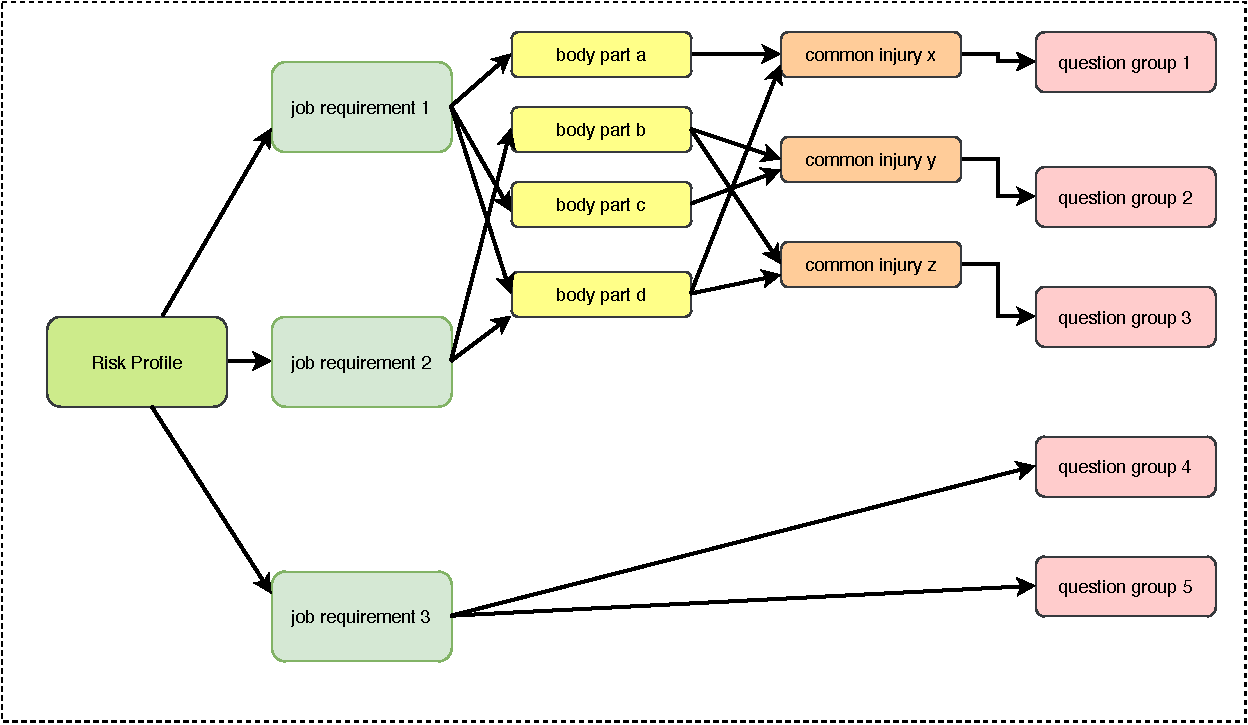
\includegraphics[width=1\columnwidth]{fig/RiskProfile.pdf}
    \label{fig:riskprofile}
\end{figure}


There are a few complications of the questionnaire that a model must adapt to. The first being its hierarchical or cascading
nature which is best described through an example.
A question could be framed asking "have you ever broken your leg?" the answer a candidate gives could be either yes/no.
If the candidate enters "yes" however this could trigger further questions about frequency, time to heal etc. and each
successive answer could themselves create a hierarchical set of questions. The other complication is the fact that answers
to questions can be of various types, for instance a simple quantity like 4, a category like 'male', a list of possible
answers, a ranking like [0-7] or a linguistic ranking like 'tall'.

Initially categorisation of a candidate will involve training an individual classification model for each role from
the answers collected through the associated questionnaire. This classification will be a binary classifier
of "suitable" or "not suitable". It is envisaged that some fuzzy categorisation of the candidate will also be
possible which will allow for a human to override a decision on the candidate who is borderline. The opportunity
to use some form of transfer or cluster learning would remove the need to train all roles separately but the initial
design will not cater for this scenario.

\subsubsection{Objective 1. To classify a candidate into a small number of groups that give a sliding suitability score.}

This objective corresponds to research question 1. To the best of my knowledge, through my literature review, no research exists that addresses the classification of closed-ended medical questionnaire's using fuzzy association rule mining. Furthermore, my literature review shows that no work has taken the predicted rule parameters from such mining and applied neural networks to fine tune the results.

\noindent
Fuzzy classification can be considered as two distinct major steps:

\noindent
\textbf{Step 1}: Create our distinct linguistic definitions to be able to describe a given domain feature in a fuzzy or non crisp manner.

In this step we introduce similarity matrix which allow us to compare two linguistic terms in a fuzzy manner. For instance suppose we had a health ranking feature (Table~\ref{tab:SimilarityMatrix}) By using this table we could say that a health ranking value of \textit{Very Poor} had a similarity of 0.5 when compared to \textit{Poor}.

\begin{table}[ht]
  \begin{center}
    \caption{Health Ranking Similarity Matrix}
    \label{tab:SimilarityMatrix}
    \begin{tabular}{|l|l|l|l|l|l|} % <-- Alignments: 1st column left, 2nd middle and 3rd right, with vertical lines in between
      \hline
      \hspace{1cm}       & \textit{Very Poor} & \textit{Poor} & \textit{Average} & \textit{Good} & \textit{Very Good} \\
      \hline
      \textit{Very Poor} & 1                  & 0.5           & 0                & 0             & 0                  \\
      \hline
      \textit{Poor}      & 0.5                & 1             & 0.5              & 0             & 0                  \\
      \hline
      \textit{Average}   & 0                  & 0.5           & 1                & 0.5           & 0                  \\
      \hline
      \textit{Good}      & 0                  & 0             & 0.5              & 1             & 0.5                \\
      \hline
      \textit{Very Good} & 0                  & 0             & 0                & 0.5           & 1                  \\
      \hline
    \end{tabular}
  \end{center}
\end{table}



Membership functions are also defined in this step. A membership function best describes the degree of truth in fuzzy logic. As an example if we were considering \textit{diastolic blood pressure} as a feature then this could be described with the membership functions shown in Figure \ref{fig:diastolic}.

% https://tex.stackexchange.com/questions/64836/change-image-size#64843
%\includegraphics[width=0.9\columnwidth]{TypesOfResearch.pdf}
\begin{figure}[!htb]
    \caption{Diastolic Blood Pressure Membership}
    \[
        \textit{DBP}_{normal}(q) = \left\{%
        \begin{array}{ll}
            1                  & \textrm{if }q<60,       \\
            \frac{60-q}{80-60} & \textrm{if }60\ge q<80. \\
        \end{array}%
        \right.
    \]

    \[
        \textit{DBP}_{high}(q) = \left\{%
        \begin{array}{ll}
            \frac{117-q}{85} & \textrm{if }90\ge q<100, \\
            1                & \textrm{if }\ge 100.     \\
        \end{array}%
        \right.
    \]
    \label{fig:diastolic}
\end{figure}


\noindent
\textbf{Step 2}: Select the most noteworthy classification rules using the linguistic definitions from step 1 along with any crisp values. This step needs to include a mechanism for handling exponential growth in noteworthy rules as the features in a domain increase.

For traditional crisp association rule mining our feature values maybe boolean or quantitative. The selection process involves finding rules that satisfy a minimum support and confidence value. So if we suppose we have a set of items

\textit{I} = \{$i_1$, $i_2$,...., $i_m$\}

\noindent
and \textit{D} represents the set of all transactions where each transaction \textit{t} is a set of items and \textit{t} $\subseteq$ \textit{I}.
% We introduce a unique identifier \textit{TID} to each transaction and 
Let \textit{A} be a set of arbitrary items in \textit{I}. A transaction \textit{t} contains \textit{A} $\iff$ \textit{A} $\subseteq$ \textit{I}. Each association rule is of the form \textit{A} $\Rightarrow$ \textit{B}, where \textit{A} $\subset$ \textit{I}, \textit{B} $\subset$ \textit{I}, and \textit{A} $\cap$ \textit{B} = $\phi$.
We can now define support (\textit{Sup}) as the percentage of transactions that contain both \textit{A} and \textit{B}

% See http://www.lsv.fr/~markey/LaTeX/doc/Mathmode.pdf
% https://oeis.org/wiki/List_of_LaTeX_mathematical_symbols

\begin{align}
    \textit{Sup}(\textit{A} \Rightarrow \textit{B}) = \frac{\mid \textit{t}_A \cap \textit{t}_B \mid}{\mid \textit{D} \mid}
    % \textit{Sup}(\textit{A} $\Rightarrow$ \textit{B}) = $\frac{\textit{t} \cap}{\textit{D}}$
\end{align}

% \begin{align}
%     \label{eq:centered}2f(x) & = \int\frac{1}{x^2}\,\mathrm{d}x3
% \end{align}

\noindent
and confidence \textit{Conf} as the percentage of transactions in \textit{D} containing \textit{A} that also contain \textit{B}.

\begin{align}
    \textit{Conf} = \frac{\textit{Sup}(\textit{A} \Rightarrow \textit{B})}{\textit{Sup}(\textit{A})} = \frac{\mid \textit{t}_A \cap \textit{t}_B \mid}{\mid \textit{t}_B \mid}
    % \textit{Sup}(\textit{A} $\Rightarrow$ \textit{B}) = $\frac{\textit{t} \cap}{\textit{D}}$
\end{align}

\noindent
Now typically in a non fuzzy approach we would introduce the Apriori algorithm which uses the
definitions for \textit{Sup} and \textit{Conf} to perform a two step procedure where itemsets are generated and tested against \textit{Sup}. The steps are:

\noindent
\textbf{Step 2.1}: set \textit{k} = 1; \textit{largeItemSet} = \textit{empty}

\noindent
\textbf{Step 2.2}: find all \textit{candidateItemsets} of size \textit{k} from original dataset

\noindent
\textbf{Step 2.3}: if a \textit{candidateItemset} transaction count is greater than \textit{Sup} then it is a frequent itemset and added to the \textit{largeItemSet}.

\noindent
\textbf{Step 2.4}: set \textit{k} = \textit{k} + 1

\noindent
\textbf{Step 2.5}: find all \textit{candidateItemsets} of size \textit{k} from \textit{largeItemSet}

\noindent
\textbf{Step 2.6}: if a \textit{candidateItemset} transaction count is greater than \textit{Sup} then it is a frequent itemset and added to the \textit{largeItemSet}.

\noindent
\textbf{Step 2.7}: if \textit{k} $\leq$ \textit{numberOfFeatures} go to Step 2.4

\noindent
\textbf{Step 2.8}: output all \textit{largeItemSet} combinations that have a confidence value larger than \textit{Conf}

\noindent
Our questionnaire data however does not only contain quantitative data and so we need to define support and confidence formula for our linguistic answers.


To date we have implemented a proof of concept of this technique that replicates the findings of Chen et al.(2008~\cite{chen2008mining}, 2009~\cite{chen2009mining}).
The solution is written in Python and uses Neo4j as a datastore, through using a more dynamic approach the implementation of our research goals should be faster to achieve.


\subsubsection{Objective 2. To define a mechanism whereby results of physical medical assessments are fed back into the system for a better predictor.}

This objective corresponds to research question 2. The physical medical assessment is outside the core architectural boundaries of the current system. There are many factors to this including geographic remoteness or the use of third party independent assessors. In order for any selected candidate to be both accurately determined and done so in a timely fashion it is vitally important that results of physical assessments are fed back into the system promptly. In fulfilling this the research will not only complete a design criteria but will also help to fill another literature gap. Chen et al. (2009~\cite{chen2009mining}) concluded that their design proved to be slow as the fuzzy membership routines were static. In feeding back this assessment information from clinical experts into the system the membership functions themselves will be altered over time and in doing so become dynamic.

To better explain this, imagine we are dealing with a crisp set, a membership function is either \textit{True} or \textit{False}, for example someone is either born in Australia or not, there is no middle ground. What about however if we wanted to specify if a person is \textit{Healthy} this is far less rigid. It could be decided on a number of factors such as they (i) can perform a set number of exercises without becoming breathless; (ii) have not visited a doctor in X years; (iii) do not consume cigarettes, alcohol or other stimulants. It is for this type of attribute that membership functions are required, they will assign a value in the range of 0 (\textit{False}) \& 1 (\textit{True}) to establish in this case how \textit{Healthy} someone is from assigning weightings to the factors (i),(ii) \& (iii) previously mentioned.

Marasini et al. (2016~\cite{marasini2016intuitionistic}) state that there are four main approaches that can be used
to define a membership function:

\begin{itemize}
    \item a "best" mathematical function
    \item a probabilistic point of view
    \item decision-theoretic approach
    \item axiomatic measurement theory
\end{itemize}

The idea of intuitionistic fuzzy sets in questionnaire analysis has been covered extensively within the work of Marasini et al. (2016~\cite{marasini2016intuitionistic}).

Kostikova et al. (2016~\cite{kostikova2016expert}) cover how dynamic membership functions maybe achieved.


\subsubsection{Objective 3. To build an anomaly detection routine to predict a list of candidates of concern.}

This objective corresponds to research question 3. The literature review has demonstrated very little research that has catered for questionnaire responses to all of Marshall's (2005~\cite{marshall2005purpose}) five data types. The main objective of this research is to use fuzzy association rule mining to improve on this situation. This objective however will endeavour to apply a number of the state of the art algorithms used in machine learning to discover rare conditions within the candidates. In completing this objective the very small pool of anomaly detection that has been applied to closed-ended questionnaire data will be enhanced. Once these anomalies are detected the research will verify if removal of such candidates leads to a better predictor of the system as a whole.

%https://au.mathworks.com/help/deeplearning/ug/create-simple-deep-learning-network-for-classification.html

We have to date implemented an anomaly detection technique originally in Octave and later ported into MATLAB. The implemented work uses a current production system that has a lot of data but lacks some integrity constraints to ensure that data is always correct.
A similar approach will be undertaken with the system currently being developed once sufficient data becomes available.

\par
\noindent
The approach can be broken down into the following steps:

\textbf{Step 1:} Select features that will be used to base our decision on whether a candidate maybe considered anomalous. Our industry partner has initially chosen BMI Banding (Table~\ref{tab:BMIBanding}), daily consumption of cigarettes, age and sex. These features should be open to change as the project evolves.

\begin{table}[ht]
  \begin{center}
    \caption{BMI Banding}
    \label{tab:BMIBanding}
    \begin{tabular}{|l|l|} % <-- Alignments: 1st column left, 2nd middle and 3rd right, with vertical lines in between
      \hline
      \textbf{BMI}            & \textbf{Banding}          \\
      \hline
      0                       & Unknown BMI               \\
      \hline
      $>~0~and~<~0.15$        & Very Severely Underweight \\
      \hline
      $\geq~0.15~and~<~0.16$  & Severely Underweight      \\
      \hline
      $\geq~0.16~and~<~0.185$ & Underweight               \\
      \hline
      $\geq~0.185~and~<~0.25$ & Normal                    \\
      \hline
      $\geq~0.25~and~<~0.30$  & Overweight                \\
      \hline
      $\geq~0.30~and~<~0.35$  & Obese Class I             \\
      \hline
      $\geq~0.35~and~<~0.40$  & Obese Class II            \\
      \hline
      $\geq~0.40~and~<~0.45$  & Obese Class III           \\
      \hline
      $\geq~0.45~and~<~0.50$  & Obese Class IV            \\
      \hline
      $\geq~0.50~and~<~0.60$  & Obese Class V             \\
      \hline
      $\geq~0.60$             & Obese Class VI            \\
      \hline
    \end{tabular}
  \end{center}
\end{table}



\textbf{Step 2:} Load, explore and clean data. The data cleansing part of this step is particularly important due to the integrity issues of the current system. The implementation removes data with poor integrity. It is at this step the distribution of a feature will be examined and all features will have their values normalised. Normalisation prevents features with a large range swamping those that do not.

\textbf{Step 3:} Define the network architecture. Whilst using the data solely from the original system it was decided not to use any type of Deep Neural Network. At this point in the research the decision was made to use both the Linear regression (Seber \& Lee, 2012~\cite{seber2012linear}) and SVM (Noble, 2006~\cite{noble2006support}) algorithms as having the ability to exclude rare occurrences was considered more important than the accuracy of those decisions. Moving forward it is the intention of the research to introduce a Deep Neural Network architecture.

% can use the following to decide upon algorithms to use

\textbf{Step 4:} Specify training options.

\textbf{Step 5:} Train the network.

The current system although lacking integrity does contain sufficient data for a classic split of the data into training, cross validation and test data. When the new system comes on line a less rigid split will need to be used involving some kind of k-fold cross validation to cater for the initial lack of data. To date some work has been done using a leave-one-out technique to gain familiarity with the approach.

\textbf{Step 6:} Predict the labels of new data and calculate the classification accuracy. Both linear regression and SVM struggled to correctly classify anomalous candidates. In total from a test population of 2834 there were actually 20 candidates rejected however our solution predicted none of these. Upon closer examination of these 20 however it became apparent that these candidates had been rejected for reasons outside of the questionnaire. For example one candidate was rejected after the assessor discovered that they had only one arm which was a question not asked through the particular job questionnaire but the job had required both arms. Other candidates were rejected for reasons that the company gave to the assessor directly and not through the questionnaire process. These findings will be fed back into giving the next iteration of the system more data integrity.


\subsubsection{Objective 4. To build a model whereby assessments maybe compared along a timeline so that assessments taken multiple times maybe analysed.}

This objective corresponds to research question 4. Chen et al. (2009~\cite{chen2009mining}) had demonstrated the inability of their research to analyse associations between questionnaire's over time. By addressing this gap this research will also benefit the industry partner's goal of comparing candidate's assessments over time. This will answer a broader question of whether a given candidate may prove unsuitable for any role or simply an individual role. One further goal of the industry partner is to allow unsuccessful candidates to be given suggestions of possible alternate rolls that they would be suitable for. This objective goes a long way to achieving this goal.

As different job roles will require the use of varying sets of questions it is paramount that we are able to in some way compare the answers for different roles in order that we may recommend am unsuccessful candidate for a more suitable role. Krusaa et al. (\cite{krusaatransfer}) propose a \textit{Questionnaire-Based Efficient Adaptive Transfer Neural Network}, QEATNN that learns to transfer knowledge between a social media and questionnaire domain. We will adapt this approach of transferring knowledge between disparate domains and instead use differing questionnaire domains.

The basic steps are:

\noindent
\textbf{Step 1:} Select representative questions from each questionnaire that are able to be transferred

\noindent
\textbf{Step 2:} Apply the work of Shi et al. (2017, \cite{shi2017local}) to create a model using Local Representative-Based
Matrix Factorisation, LRMF that splits the representative questions into global (global attributes) and local (personal attributes) representatives.

\noindent
\textbf{Step 3:} Deduce whether sufficient local representatives of an unsuccessful candidate from one questionnaire domain match those of a successful candidate from another domain and if so recommend this candidate for the alternate role.

\subsection{Demonstrate the artefact can be used to help solve the focal problem}

Figure~\ref{fig:specificjobrequirement} demonstrates a more specific job requirement for lifting heavy weights from floor
to waist. It has been partially completed for the purpose of explanation only and does not represent a genuine scenario.
Of particular note are the edges for heavy weight,
hip and flexor. It is on these edges that properties will initially be attached such as the value for the actual weight
considered "heavy" by an expert in the field. As our classifier begins to acquire data it is these properties that will
dynamically be altered in order to solve our core problem of classifying a candidate. An added bonus of the classifier
will be the ability to suggest alternate candidate roles to an unsuccessful candidate that they may be suitable for.

% https://tex.stackexchange.com/questions/64836/change-image-size#64843
%\includegraphics[width=0.9\columnwidth]{TypesOfResearch.pdf}
\begin{figure}[!htb]
    \caption{Specific Job Requirement}
    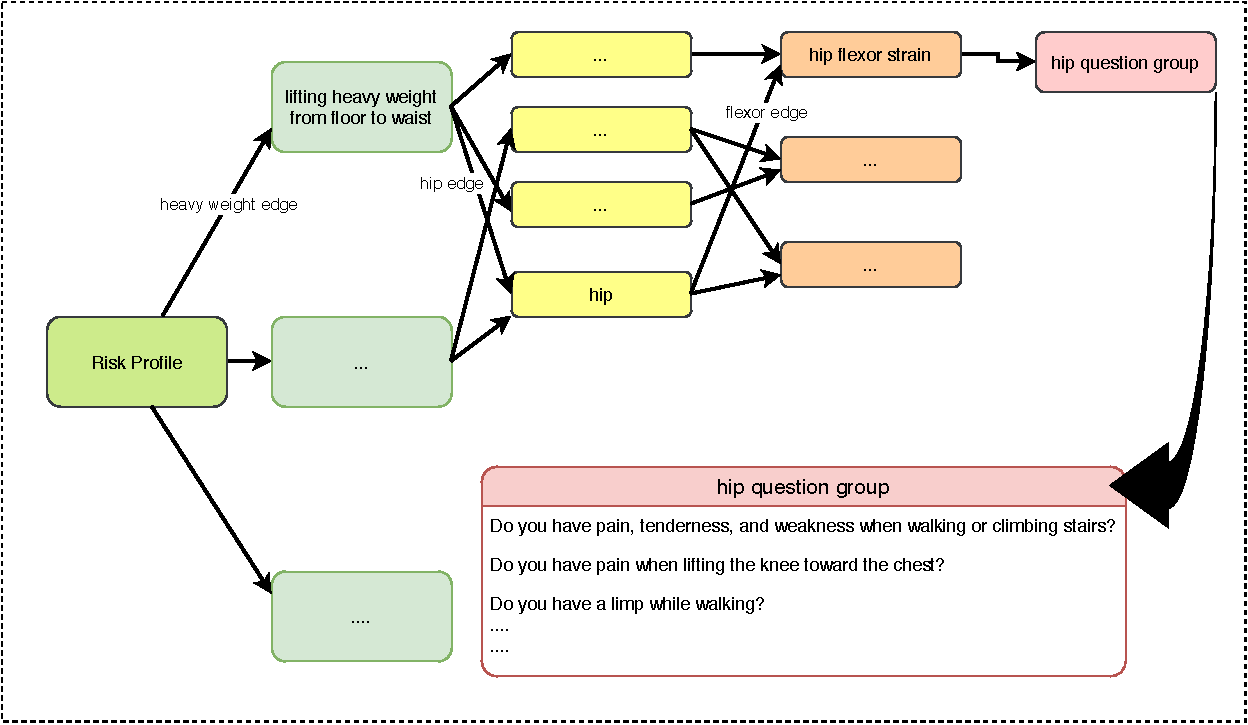
\includegraphics[width=1\columnwidth]{fig/SpecificJobRequirement.pdf}
    \label{fig:specificjobrequirement}
\end{figure}



\subsection{Evaluate how well the artefact solves the focal problem}

Objective 5 of Section~\ref{sec:disObjectives} discusses evaluation of the developed artefacts and in so doing satisfies
this requirement of Peffers et al. described in the Methodology Section \ref{sec:disMethodology}.

\subsubsection{Objective 5. To evaluate the developed artefacts from the previous objectives.}

This objective corresponds to research question 5. For our classification objective there are a number of typical tests to indicate the correctness of a classification and these include amongst other measures confusion matrix, area under the ROC curve and F1 score.

%Evaluation should state what success looks like, for instance, objective 1 may be successful if we can flag 60\% of candidates of concern. Or our prototype should show improved learning through assessor feedback.

% https://towardsdatascience.com/how-to-measure-the-goodness-of-a-regression-model-60c7f87614ce
%https://medium.com/analytics-vidhya/evaluation-metrics-in-machine-learning-models-using-python-fb6199450fba
% https://towardsdatascience.com/accuracy-precision-recall-or-f1-331fb37c5cb9


Briefly if we are describing a binary classification such as the candidate is "suitable" or "not suitable" we can plot a confusion matrix of the form shown in Fig~\ref{fig:ConfusionMatrix}. From this matrix we can calculate attributes such as accuracy, precision and recall to decide whether our results have been noteworthy. The reader may at this point believe that to be noteworthy we should simply strive for the highest accuracy in our classification but that may not always be the case. For instance we may gain an accuracy of over 98\% but if we ultimately select a candidate who would have been rejected if given a physical assessment then this could present an unforeseen cost to the client and also a loss of faith in the predictor. This then brings us to the other two attributes precision and recall which represent the ratio of true positives in the model to the predicted positives and actual positives respectively. Precision should be closely watched when the cost of a false positive is high and recall when the cost of a false negative is high.

Initially all of our candidates will have a medical assessment and so the cost of a false positive will not truly be of concern. That does not however mean that our success of a classification for this research should only look at accuracy as eventually the medical assessor should not need to be called upon for every situation. It does however offer some flexibility in deciding the success criteria at this stage of the research.

\begin{figure}[h]
    \caption{Confusion matrix} \label{fig:ConfusionMatrix}
    \begin{tabular}{|l|l|l|}
        \hline
                                          & \textbf{Suitable (Actual)} & \textbf{Not Suitable (Actual)} \\ \hline
        \textbf{Suitable (Predicted)}     & TP (True Positive)         & FP (False Positive)            \\ \hline
        \textbf{Not Suitable (Predicted)} & FN (False Negative)        & TN (True Negative)             \\ \hline
    \end{tabular}

    % https://www.latex-tutorial.com/tutorials/amsmath/
    \begin{align*}
        accuracy  & = \frac{(TP+TN)}{(TP+TN+FP+FN)} \\
        precision & = \frac{TP}{(TP+FP)}            \\
        recall    & = \frac{TP}{(TP+FN)}            \\
    \end{align*}

\end{figure}


% https://www.displayr.com/what-is-a-roc-curve-how-to-interpret-it/
\noindent
Fawcett (2006~\cite{fawcett2006introduction}) explains the intricacies of an ROC graph, an example of which, is shown in Fig~\ref{fig:ROCCurve}. It is a very visual means by which the correctness of a classifier can be judged by varying the threshold. The threshold being a value between 0\% and 100\%, that is used to set the limit to decide upon which class an instance belongs to. In our case, we will classify a candidate as either "suitable" or "not suitable". The graph plots the true positive rate against the false positive rate. For us the true positive rate is the rate in which candidates are correctly identified as "suitable" for the job role in question. A classifier that approaches the top left of the graph is considered a better classifier than one further away. The closer the curve comes to the "random" 45 degree line the less accurate the classifier and this would equate to using a "coin toss" to decide upon the candidates suitability. Although an ROC graph is a very visual tool, to evaluate multiple classifiers the approach used is to take the area under the ROC curve (AUC). Generally, although not always true, a high AUC score is a better predictor than one that is lower. One advantage that an ROC graph has over a confusion matrix is that it does not depend on class distribution and hence is still suitable for evaluating classifiers that contain rare or anomalous values.

%cSpell:disable
%\documentclass{article}
%\usepackage[margin=0in,paperheight=3.9in,paperwidth=6.3in]{geometry}
%\usepackage[dvipsnames]{xcolor}
%\usepackage{pgfplots}
%\pgfplotsset{width=30cm,compat=1.9}
%\usetikzlibrary{patterns}

%\begin{document}
\begin{figure}[!htb]
  \caption{ROC graph} \label{fig:ROCCurve}
  \begin{tikzpicture}
    \begin{axis}
      [
        xlabel={False Positive Rate  (1- Specificity) \%}, ylabel={True Positive Rate (Sensitivity) \%}, xmin=0.0, xmax=100,
        ymin=0.0, ymax=100,
        height=10cm,
        width=15cm,
        legend columns=5,
        legend pos=north east,
        ticklabel style = {font=\large},
        label style = {font=\large},
        xtick={0, 20, 40, 60, 80, 100},
        ytick={0, 20, 40, 60, 80, 100},
      ]

      \addplot
      [
        line width=1pt,
        color=green,
        mark=square,
      ]
      coordinates{
          (0.0, 0.0) (0.0, 5) (0.0, 10) (0.0, 15) (0.0, 20) (0.0, 25) (0.0, 35) (0.0, 45) (0.4, 55) (1, 65) (2, 77) (3.5, 85) (4.5, 87)
          (5.5, 89)  (6.7, 92) (8.4, 94) (14, 97)
          (20, 98.5) (30, 100) (40, 100) (50, 100) (60, 100) (70, 100) (80, 100) (90, 100) (100, 100)};

      \addplot
      [
        line width=1pt,
        color=RedViolet,
        mark=halfsquare*,
      ]
      coordinates{
          (0.0, 0.0) (20, 20) (40, 40) (60, 60) (80, 80) (100, 100) };

      \legend{$ROC$,$Random$}
    \end{axis}
  \end{tikzpicture}

  \begin{align*}
    True Positive Rate  & = \frac{TP}{(TP+FN)} \\
    False Positive Rate & = \frac{FP}{(TP+FN)} \\
  \end{align*}

\end{figure}

%\end{document}
%cSpell:enable

The final success indicator that we will employ is the F1 score. This score is based on the precision and recall values mentioned in Fig~\ref{fig:ConfusionMatrix}

\begin{align*}
    F1 & = 2 * \frac{Precision*Recall}{Precision+Recall} \\
\end{align*}

It is used when a balance is required between precision and recall. The reason for the F1 score over using straight accuracy is that accuracy is affected highly by true negatives which are not often a focus in business problems. False negatives and positives usually claim the majority of the focus as they are responsible for most of the cost involved in incorrect classification. Thus the F1 score seeks to find balance between precision and recall when there is an uneven class distribution.


\subsection{Communicate the outcomes of the research}


Amongst the outcomes of this research will be the development of a number of novel algorithms to be incorporated into a commercial software product. It is the algorithms that are developed during the design phase that will satisfy the artefact requirement of DSR. The stakeholder community will initially involve the industry partner of the university but will ultimately be useful to anyone dealing with the problem of classifying the answers to closed survey/questionnaire data.
\par
Through progressing the research to completion the communication of the outcomes will satisfy the industry partner. The wider research
community will become aware of the outcomes through publishing one or two papers at recognised conferences.





\section{Future Impact/Significance}\label{sec:disFutureImpact}

%Each objective is expected to make a significant contribution to the aim or aims. While it should straightforward to tie the aims of your project to the central thesis statement, it can be trickier to tie the objectives to the aims. This is what your significance section needs to set out.

%\begin{itemize}
%	\item The thesis is important to the reader (the stakeholder)
%	\item Achieving the aims supports the thesis
%	\item Achieving the objectives supports the aims
%\end{itemize}


The significance of this research will be described both from a theoretical and practical standpoint.

\subsection{Theoretical significance:}

The findings from this study contribute to the machine learning community by addressing some areas of misrepresentation of the closed-data questionnaire. Specifically this research sets out to address the problem of handling a range of different response data types all at the same time by introducing a fuzzy association rule mining approach. Although fuzzy ARM has been looked at in a very small number of papers they have neither found a solution to the time consuming task of creating membership functions statically nor attempted to improve upon the results by tuning the rule parameters using gradient descent. The research will also enrich the understanding of analysing questionnaire responses along a timeline.  

\subsection{Practical significance:}

Providing unnecessary medical assessments to candidates that are unsuitable for a role raises a number of issues to the selection process of our industry partner


\begin{itemize}
	\item The cost of providing the assessment can be prohibitive.
	\item As the candidate put forward for an assessment is usually a long way through the selection process suitable secondary candidate's are not always available. This may be because the other candidate has already found a new role. This can also lead to the even larger problem of having to initiate the candidate recruitment cycle all over starting with the initial interview stage. 
	\item The candidate that is unsuitable for the role may well be suitable for a different role but has now missed the opportunity to apply for that role.
\end{itemize}


% Example
%To date there has been little consideration of EIT in regimes with widely mismatched probe and coupling fields (Aim 1); exploring a solution, via a theoretical model, to the understanding of whether non-optical fields can control absorption (Objective 1) will open up feasibility studies of future low-power, compact experimental system useful for future quantum control systems.The development of such a system (Aim 2) will be underpinned by the first verification that EIT is possible in a widely mismatched system in rubidium vapour(Objective 2).To fully verify the model developed in Objective 1, polarization effects will be explored (Objective 3) with the goal of delivering finer control of the absorption of the probe beam via field control that is not dependent on changing the wavelength (Aim 3).

\pagebreak

\section{Research Timeline}\label{sec:disResearchTimeline}
The following represents a guide to the expected duration of each activity in this research study.

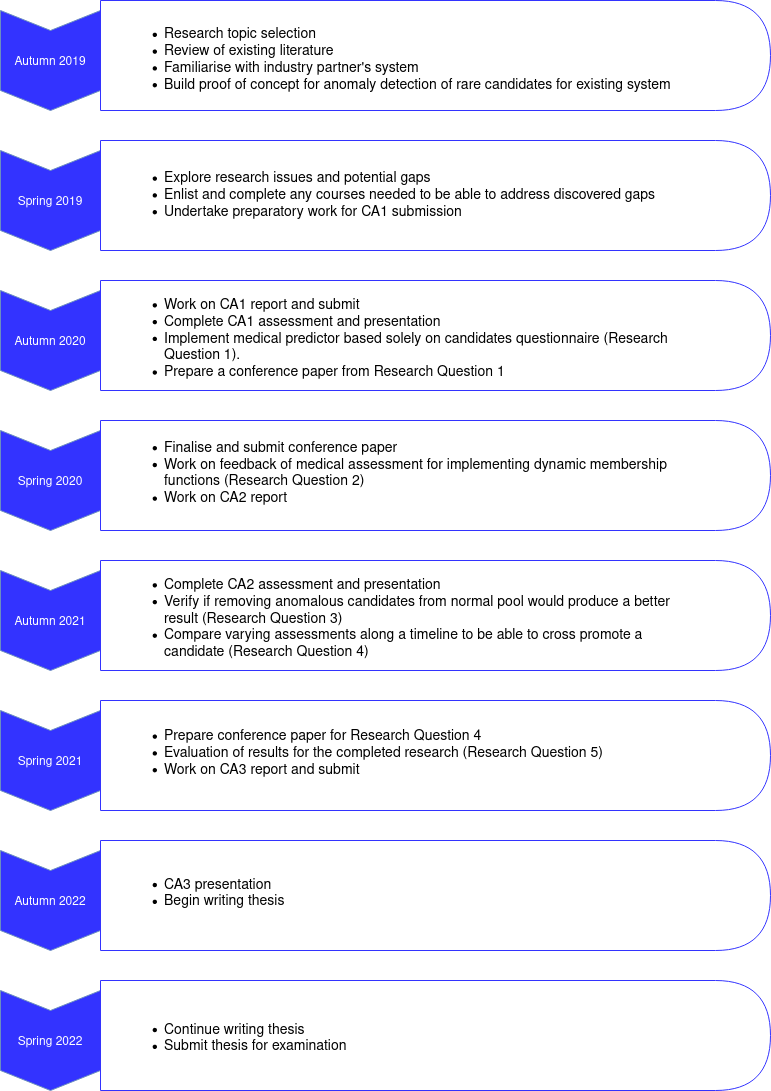
\includegraphics[scale=0.5]{fig/ResearchTimeline.png}















%%%\chapter{Introduction}\label{ch:Intro}

\section{Background}\label{sec:Background} 
In order to define the issue of ``classification imbalance'' it may be helpful to firstly describe what the break up of various classes within a dataset need to be in order for that dataset to be considered ``imbalanced'' and then to describe some real world examples of problems that exhibit such an imbalance. The title of this paper refers to ``accuracy'' or more precisely predictive accuracy and within a reasonably balanced dataset this would be a good measure. However, in an imbalanced situation it is more usual to see an ROC curve or something similar used to rate whether the classification has been ``accurate'' (Ling \& Li, 1998~\cite{ling1998data}; Drummond \& Holte, 2000~\cite{drummond2000explicitly} Provost \& Fawcett, 2001~\cite{provost2001robust}; Bradley 1997~\cite{bradley1997use}).  
\par
Describing class break up, He and Garcia (2008~\cite{he2008learning}) refer to the ideal situation where a classifier would be split evenly within any given domain problem. However, such a situation is rare and more often than not we find a disproportionately skewed set of classifiers. Their work suggests that an imbalanced problem would have a percentage range from a (majority~/~minority) class split of anywhere between (90\%~/~10\%) and (\textgreater=99\%~/~\textless=1\%). In fact, the research community as a whole regularly sees class imbalances of 100:1, 1000:1 and 10000:1. 
\par
When it comes to real world examples of class imbalance, fraud detection in the use of credit cards is a classic example where the percentage of fraudulent usage is a tiny fraction of a percent compared to its honest counterpart. Another example of an imbalance scenario is from the theft of electricity worldwide. It is suggested that this form of theft rates in the top five forms of theft globally. Utility companies are faced with a situation where less than 2\% of usage classification is fraudulent, yet it represents a very sizeable dent in their profit.
\par
\secref{ch:LSurvey} contains an extensive literature review, the aim of which is to critique an exhaustive collection of deep learning methods that address the issue of class imbalance. The approach taken is based on the guidelines suggested by Kitchenham \& Charters (2010~\cite{Kitchenham2010}), a preliminary SLR approach was used to address the research questions at hand.
\par
Within the UTS online library the following electronic scientific databases were chosen to reveal the literature required for this review:

\begin{itemize}
    \item Computers \& Applied Sciences Complete(EBSCO) (\href{https://www.ebsco.com/}{https://www.ebsco.com/})
    \item Google Scholar (\href{https://www.scholar.google.com.au/}{https://www.scholar.google.com.au/})
	\item IEEE Xplore (\href{https://www.ieexplore.ieee.org/Xplore/}{https://www.ieexplore.ieee.org/Xplore/})
    \item ProQuest Science and Technology (\href{https://www.proquest.com/}{https://www.proquest.com/})
    \item Science Direct (Elsevier) (\href{https://www.sciencedirect.com/}{https://www.sciencedirect.com/})
    \item Scopus (Elsevier) (\href{https://www.scopus.com}{https://www.scopus.com})
    \item SpringerLink (\href{https://link.springer.com/}{https://link.springer.com/})
\end{itemize}

The search strings used to find out the relevant literature were "class imbalance", "deep learning", "neural networks", "deep neural networks", "class rarity", "class minority" and "skewed data". 

From this list certain papers were removed based upon the following criteria:

\begin{itemize}
    \item Look at only low levels of imbalance
    \item Only have a single dataset for evaluation as this is considered too niche
    \item Imbalance is not the primary goal of the research 
\end{itemize}

\section{Research Objectives}\label{sec:RObj} 

The aims of the project are to:
\renewcommand{\theenumi}{\roman{enumi}}
\begin{enumerate}
\item review traditional machine learning techniques to handle class imbalance. 
\item review deep learning techniques to handle class imbalance. 
\item make a list of public datasets showing correlation to our industry dataset. 
\item apply review findings to these public non image datasets. 
\item apply review findings to existing industry dataset. 
\end{enumerate}

\section{Thesis Organization}\label{sec:ThOrg} 
This thesis is organised as follows:

\begin{itemize}
\item {\it Chapter 2}: This chapter presents a literature review of the current research into classification imbalance in both a traditional and deep learning manner

%\item {\it Chapter 3}: ... are derived in this chapter.

%\item {\it Chapter 4}: This chapter presents ...

%\item {\it Chapter 5}: A brief summary of the thesis contents and its contributions are given in the final chapter. Recommendation for future works is given as well.
\end{itemize}











%%%\chapter{Literature Review}\label{ch:LSurvey}

%\section{Style}\label{sec:Style}
%This review is organised in what is considered a 'Classic' style whereby it will be drawing much of its content from the major writings in the field of classification imbalance. 

%\section{Aim}\label{sec:Aim}
%The aim of the review is to describe the best in class methods currently available to a researcher to overcome the issue of classification imbalance. Although the field is a comparatively new one there has been a great number of papers written on the subject with a large number of suggestions for ``gaps'' within it. The review starts its journey following the work of Leevy et Al \cite{leevy2018survey} and Japkowicz and Stephen \cite{Japkowicz2002} which act as a springboard into a number of important 'benchmark' studies and articles about classification imbalance.


%\section{Scope}\label{sec:Scope}
%In reviewing potential methods to reduce the effects of the classification imbalance problem, it will not be the job of this work to somehow give a definitive rating for each of the methods to any given classification problem. It is hoped however, that for the dataset being used we will be able to within reason suggest the most appropriate one. This work will also not attempt to study the imbalance issue within a multi classification problem as this is seen as a variation on a theme of having multiple binary classification problems. 


%\section{Definition of classification imbalance}\label{sec:Defn}

%\textit{The literature review starts with an introduction or series of introductory paragraphs which provides for the reader the content being covered, the structure or how the review is organised, and the delimitation (or boundaries) of the subject matter to be covered (mentions what is outside the scope of the study).}

%In order to define the issue of ``classification imbalance'' it may be helpful to firstly describe what the break up of various classes within a dataset need to be in order for that dataset to be considered ``imbalanced'' and then to describe some real world examples of problems that exhibit such an imbalance.  
%\par
%With regard to class break up, He and Garcia \cite{he2008learning} refer to the ideal situation where a classifier would be split evenly within any given domain problem. However such a situation is rare and more often than not we find a disproportionately skewed set of classifiers. Their work suggests that an imbalanced problem would have a percentage range from a (majority~/~minority) class split of anywhere between (90\%~/~10\%) and (\textgreater=99\%~/~\textless=1\%). In fact the research community as a whole regularly sees class imbalances of 100:1, 1000:1 and 10000:1. 
%\par
%When it comes to real world examples of class imbalance, fraud detection in the use of credit cards is a classic example where the percentage of fraudulent usage is a tiny fraction of a percent compared to its honest counterpart. Another example of an imbalance scenario is from the theft of electricity worldwide. It is suggested that this form of theft rates in the top five forms of theft globally. Utility companies are faced with a situation where less than 2\% of usage classification is fraudulent yet it represents a very sizeable dent in their profit.

% \section{Why classification imbalance occurs}\label{sec:Why}
\section{Introduction}\label{sec:Why}

% \textit{The literature review has a body consisting of series of sections and sub-sections which discuss the literature in a logical and coherent way.Each section discusses and evaluates the literature in terms of the most important topics or key concepts relevant to the area of study in which you are working.Each section ends with a summary and sentences which relate this to the focus of the research area.The body paragraphs should be well organised and structured. See our resources on effective paragraph writing.}

He and Garcia (2008~\cite{he2008learning}) refer to the idea of intrinsic-based and extrinsic-based class imbalances. Intrinsic being the occurrence of a class skew due to the data itself and extrinsic being a possible skew due to reasons beyond the data. Examples of intrinsic imbalance include picking out the hopefully small number of spam emails from the multitude of daily emails received so that the recipient is not inconvenienced but also does not miss any email. Another would be in predicting ``churn'' within an insurer`s member base, the vast majority of members would usually roll their policy over around its renewal time but a small percentage would switch. The insurer needs to target these potential churners before they make their decision but in targeting too many of the members they run the risk of alienating more than they can hope to retain. An example of extrinsic imbalance being a break in the recording of the data brought about through some type of interruption. Another being the data is collected at set times within which the minority class is most prevalent. Physical failures such as power supply or storage space may also create artificial skews in the data. A final example of extrinsic imbalance being manifested due to a change in the process of gathering of the actual data. 
\par
Although this work makes no distinction between intrinsic and extrinsic imbalance, it is the authors belief that extrinsic imbalance issues will prove to be very relevant to this work's existing industry dataset. The data collection process has changed over a number of years and is reliant on a repeatable standard line of enquiry from a human practitioner. As time moves on, practitioners change and if the standards are not strictly adhered to then over time the data becomes skewed through no other reason than change in interpretation. That being said intrinsic imbalance is also present within the dataset through the simple fact that some candidate's attributes will be underrepresented within the total pool. 

% \section{Traditional class imbalance}

%[TODO explain RF etc and cite some papers]

\section{Traditional Methods}\label{sec:TradMethods}
Possible solutions to the traditional class imbalance issue are typically split into data level and algorithm level solutions as described in the work of Ali et al. (2015~\cite{ali2015classification}). The data level encompassing both data sampling and feature selection methods whilst the algorithm level includes cost sensitive and hybrid or ensemble applications. 
\par
Typical data sampling, cost sensitive techniques include Random Over-Sampling (ROS) and Random-Under Sampling (RUS). Whereas typical algorithm level methods include amongst others fuzzy rule-based classification (Chi et al., 1996~\cite{chi1996fuzzy}).
\par
Over sampling described in \secref{subsec:OverSampling} and under sampling in \secref{subsec:UnderSampling} can be thought of as two sides of the same coin in that over-sampling involves expanding the minority class through repetition and thus increasing the occurrence of the class whereas under-sampling involves removing samples from the majority class and hence reducing its dominance on the overall classification. Whereas entries of the minority class maybe added either randomly or through some computed method the entries from the majority class tend to be removed randomly. In fact the process of adjusting the majority/minority class has been the subject of a lot of work in its own right (Khoshgoftaar et al., 2007  \cite{khoshgoftaar2007learning}; Van Hulse et al., 2007 \cite{van2007experimental}).
\par
Finally it should be remembered that although til now the reader may have assumed that it is possible to improve classification results at either the data or algorithm level the hybrid scenario is one in which some combination of both of these may help. One example of this would be the introduction of the Random Forest (RF) classifier which although based on the earlier Random Decision Forest also has the inclusion of Bagging techniques (Gislason et al., 2006 \cite{gislason2006random}). 

\subsection{Over sampling}\label{subsec:OverSampling}
Two prevalent over sampling techniques are Random Over Sampling (ROS) (Zhang \& Li, 2014~\cite{zhang2014rwo}) and Synthetic Minority Over-Sampling Technique (SMOTE)  (Chawla et al., 2002~\cite{chawla2002smote}; Chawla et al., 2003 \cite{chawla2003smoteboost}; Han Wang \& Mao \cite{han2005borderline}). One common complaint of over sampling techniques is their propensity to create an ``over-fitting'' (Fig~\ref{fig:Oversampling}) issue whereby the training data is too heavily mimicked leading to a poor model predictor. This over-fitting concern however can be mostly overcome through the use of SMOTE (Fern\'{a}ndez et al., 2017~\cite{fernandez2017insight}). Another complaint is an even larger training dataset than initially considered useful. In looking at the amount to which a minority class should be inflated it may appear reasonable that obtaining a 50/50 split would be ideal but Japkowicz and Stephen (2002~\cite{Japkowicz2002}), Fawcett and Provost (1997~\cite{fawcett1997adaptive}) along with Estabrooks and Japkowicz (2001~\cite{estabrooks2001mixture}) offer a counter argument and show that such a split would not produce the most favourable results.

\tikzset{every picture/.style={line width=0.75pt}} %set default line width to 0.75pt        
\begin{figure}[htbp]
\centering

\begin{tikzpicture}[x=0.75pt,y=0.75pt,yscale=-1,xscale=1]
%uncomment if require: \path (0,300); %set diagram left start at 0, and has height of 300

%Shape: Axis 2D [id:dp33720031646484827] 
\draw  (50,215.2) -- (289.5,215.2)(73.95,37) -- (73.95,235) (282.5,210.2) -- (289.5,215.2) -- (282.5,220.2) (68.95,44) -- (73.95,37) -- (78.95,44)  ;
%Straight Lines [id:da49156386348114545] 
\draw [color={rgb, 255:red, 144; green, 19; blue, 254 }  ,draw opacity=1 ][fill={rgb, 255:red, 144; green, 19; blue, 254 }  ,fill opacity=1 ][line width=1.5]    (119,76) -- (219,176) ;


%Shape: Axis 2D [id:dp9978017465833935] 
\draw  (369,214.2) -- (608.5,214.2)(392.95,36) -- (392.95,234) (601.5,209.2) -- (608.5,214.2) -- (601.5,219.2) (387.95,43) -- (392.95,36) -- (397.95,43)  ;
%Curve Lines [id:da10887800526684499] 
\draw [color={rgb, 255:red, 144; green, 19; blue, 254 }  ,draw opacity=1 ][line width=1.5]    (408.5,111) .. controls (439.5,98) and (483.5,120) .. (522.5,204) ;



% Text Node
\draw (134,60) node  [align=left] {o};
% Text Node
\draw (154,80) node  [align=left] {o};
% Text Node
\draw (182,100) node  [align=left] {o};
% Text Node
\draw (180,63) node  [align=left] {o};
% Text Node
\draw (202,85) node  [align=left] {o};
% Text Node
\draw (217,110) node  [align=left] {o};
% Text Node
\draw (208,127) node  [align=left] {o};
% Text Node
\draw (231,147) node  [align=left] {o};
% Text Node
\draw (258,125) node  [align=left] {o};
% Text Node
\draw (253,168) node  [align=left] {o};
% Text Node
\draw (243,89) node  [align=left] {o};
% Text Node
\draw (208,57) node  [align=left] {o};
% Text Node
\draw (154,54) node  [align=left] {o};
% Text Node
\draw (182,80) node  [align=left] {o};
% Text Node
\draw (223,74) node  [align=left] {o};
% Text Node
\draw (239,125) node  [align=left] {o};
% Text Node
\draw (266,146) node  [align=left] {o};
% Text Node
\draw (228,93) node  [align=left] {o};
% Text Node
\draw (120,126) node [color={rgb, 255:red, 208; green, 2; blue, 27 }  ,opacity=1 ] [align=left] {x};
% Text Node
\draw (140,146) node [color={rgb, 255:red, 208; green, 2; blue, 27 }  ,opacity=1 ] [align=left] {x};
% Text Node
\draw (167,170) node [color={rgb, 255:red, 208; green, 2; blue, 27 }  ,opacity=1 ] [align=left] {x};
% Text Node
\draw (453,59) node  [align=left] {o};
% Text Node
\draw (473,79) node  [align=left] {o};
% Text Node
\draw (501,99) node  [align=left] {o};
% Text Node
\draw (499,62) node  [align=left] {o};
% Text Node
\draw (521,84) node  [align=left] {o};
% Text Node
\draw (536,109) node  [align=left] {o};
% Text Node
\draw (527,126) node  [align=left] {o};
% Text Node
\draw (550,146) node  [align=left] {o};
% Text Node
\draw (577,124) node  [align=left] {o};
% Text Node
\draw (572,167) node  [align=left] {o};
% Text Node
\draw (562,88) node  [align=left] {o};
% Text Node
\draw (527,56) node  [align=left] {o};
% Text Node
\draw (473,53) node  [align=left] {o};
% Text Node
\draw (501,79) node  [align=left] {o};
% Text Node
\draw (542,73) node  [align=left] {o};
% Text Node
\draw (558,124) node  [align=left] {o};
% Text Node
\draw (585,145) node  [align=left] {o};
% Text Node
\draw (547,92) node  [align=left] {o};
% Text Node
\draw (439,125) node [scale=2.488,color={rgb, 255:red, 208; green, 2; blue, 27 }  ,opacity=1 ] [align=left] {x};
% Text Node
\draw (459,145) node [scale=2.488,color={rgb, 255:red, 208; green, 2; blue, 27 }  ,opacity=1 ] [align=left] {x};
% Text Node
\draw (486,169) node [scale=2.488,color={rgb, 255:red, 208; green, 2; blue, 27 }  ,opacity=1 ] [align=left] {x};


\end{tikzpicture}

\caption{Oversampling} \label{fig:Oversampling}
\end{figure}


\subsection{Under sampling}\label{subsec:UnderSampling}
One of the most used under sampling (Fig~\ref{fig:Undersampling}) techniques is Random Under Sampling (RUS) (Seiffert et al., 2009~\cite{seiffert2009rusboost}). Good practice in the removal process from the majority class is that the data removed lies as far away from any boundary with the minority class as possible. Practitioners point out that one of the disadvantages of under sampling is the possible removal of valuable information from the core set and a possible change in the majority class's distribution if care is not taken in the extraction. For instance we could remove a large portion of young people from an otherwise well distributed cohort of data. 




\tikzset{every picture/.style={line width=0.75pt}} %set default line width to 0.75pt       
\begin{figure}[htbp]
\centering


\begin{tikzpicture}[x=0.75pt,y=0.75pt,yscale=-1,xscale=1]
%uncomment if require: \path (0,300); %set diagram left start at 0, and has height of 300

%Shape: Axis 2D [id:dp33720031646484827] 
\draw  (50,215.2) -- (289.5,215.2)(73.95,37) -- (73.95,235) (282.5,210.2) -- (289.5,215.2) -- (282.5,220.2) (68.95,44) -- (73.95,37) -- (78.95,44)  ;
%Straight Lines [id:da49156386348114545] 
\draw [color={rgb, 255:red, 144; green, 19; blue, 254 }  ,draw opacity=1 ][fill={rgb, 255:red, 144; green, 19; blue, 254 }  ,fill opacity=1 ][line width=1.5]    (119,76) -- (219,176) ;


%Shape: Axis 2D [id:dp9978017465833935] 
\draw  (369,214.2) -- (608.5,214.2)(392.95,36) -- (392.95,234) (601.5,209.2) -- (608.5,214.2) -- (601.5,219.2) (387.95,43) -- (392.95,36) -- (397.95,43)  ;
%Straight Lines [id:da6705581541742359] 
\draw [color={rgb, 255:red, 144; green, 19; blue, 254 }  ,draw opacity=1 ][fill={rgb, 255:red, 144; green, 19; blue, 254 }  ,fill opacity=1 ][line width=1.5]    (428,91) -- (580.5,153) ;



% Text Node
\draw (134,60) node  [align=left] {o};
% Text Node
\draw (154,80) node  [align=left] {o};
% Text Node
\draw (182,100) node  [align=left] {o};
% Text Node
\draw (180,63) node  [align=left] {o};
% Text Node
\draw (202,85) node  [align=left] {o};
% Text Node
\draw (217,110) node  [align=left] {o};
% Text Node
\draw (208,127) node  [align=left] {o};
% Text Node
\draw (231,147) node  [align=left] {o};
% Text Node
\draw (258,125) node  [align=left] {o};
% Text Node
\draw (253,168) node  [align=left] {o};
% Text Node
\draw (243,89) node  [align=left] {o};
% Text Node
\draw (208,57) node  [align=left] {o};
% Text Node
\draw (154,54) node  [align=left] {o};
% Text Node
\draw (182,80) node  [align=left] {o};
% Text Node
\draw (223,74) node  [align=left] {o};
% Text Node
\draw (239,125) node  [align=left] {o};
% Text Node
\draw (266,146) node  [align=left] {o};
% Text Node
\draw (228,93) node  [align=left] {o};
% Text Node
\draw (120,126) node [color={rgb, 255:red, 208; green, 2; blue, 27 }  ,opacity=1 ] [align=left] {x};
% Text Node
\draw (140,146) node [color={rgb, 255:red, 208; green, 2; blue, 27 }  ,opacity=1 ] [align=left] {x};
% Text Node
\draw (164,167) node [color={rgb, 255:red, 208; green, 2; blue, 27 }  ,opacity=1 ] [align=left] {x};
% Text Node
\draw (453,59) node  [align=left] {o};
% Text Node
\draw (473,79) node  [align=left] {o};
% Text Node
\draw (499,62) node  [align=left] {o};
% Text Node
\draw (521,84) node  [align=left] {o};
% Text Node
\draw (562,88) node  [align=left] {o};
% Text Node
\draw (527,56) node  [align=left] {o};
% Text Node
\draw (473,53) node  [align=left] {o};
% Text Node
\draw (501,79) node  [align=left] {o};
% Text Node
\draw (542,73) node  [align=left] {o};
% Text Node
\draw (547,92) node  [align=left] {o};
% Text Node
\draw (443,124) node [color={rgb, 255:red, 208; green, 2; blue, 27 }  ,opacity=1 ] [align=left] {x};
% Text Node
\draw (464,145) node [color={rgb, 255:red, 208; green, 2; blue, 27 }  ,opacity=1 ] [align=left] {x};
% Text Node
\draw (487,162) node [color={rgb, 255:red, 208; green, 2; blue, 27 }  ,opacity=1 ] [align=left] {x};


\end{tikzpicture}

\caption{Undersampling} \label{fig:Undersampling}
\end{figure}

\subsection{Feature selection}
Feature selection is the process of selecting the most influential features for a given dataset to produce an improved classification process. While not solely related to imbalance conditions a consequence of better feature selection usually leads the betterment of the effects of such imbalances (Yin et al., 2013~\cite{yin2013feature}; Mladenic \& Grobelnik, 1999~\cite{mladenic1999feature}). A downside of using feature selection to reduce imbalance is the extra computational load that is required. The work undertaken by Mladenic and Grobelnik (1999~\cite{mladenic1999feature}) rates a number of feature selection ideas and puts the ``odds ratio'' ahead of the rest. This is confirmed in the work by Zhang et al (2018~\cite{zhang2018image}). This rating however is not confirmed in some works and the general belief is that feature selection is very much a case by case situation.

\subsection{Cost sensitive methods}
The general premise of cost sensitive methods is to assign a higher weight or prominence to a given occurrence of a minority classification than any majority one so as to boost the worth of the minority classifier and reduce the effects of any imbalance. Domingos (1999~\cite{domingos1999metacost}) and Elkan (2001~\cite{elkan2001foundations}) are early studies on this important topic. They rely upon something called a cost matrix (Table~\ref{tab:costmatrix}) which encapsulates all possible outcomes of a two class problem.

\begin{table}[htbp]
\centering
\begin{tabular}{|l|c|c|}
\hline
                 & \multicolumn{1}{l|}{actual negative} & \multicolumn{1}{l|}{actual positive} \\ \hline
predict negative & C(0, 0)                              & C(0, 1)                              \\ \hline
predict positive & C(1, 0)                              & C(1, 1)                              \\ \hline
\end{tabular}
\caption{Cost Matrix}
\label{tab:costmatrix}
\end{table}

 
An example given by Elkan (2001~\cite{elkan2001foundations}) of such a cost matrix would be in attempting to find a fraudulent credit card transaction (Table~\ref{tab:costmatrix_cc_example}). In this scenario approval of a fraudulent transaction would cost the provider the total amount or \textit{``-x''} whereas refusing the legitimate transaction would damage the provider's reputation with the client. Here Elkan suggests an arbitrary \$20 loss to be sufficient. Refusing a fraudulent transaction he attributes a \$20 benefit and finally a legitimate approval will cost the institution 2\% of the cost of the total amount or \textit{``x''}.

\begin{table}[htbp]
\centering
\begin{tabular}{|l|c|c|}
\hline
                 & \multicolumn{1}{l|}{fraudulent} & \multicolumn{1}{l|}{legitimate} \\ \hline
refuse & \$20                              & -\$20                              \\ \hline
approve & -x                              & -0.02x                              \\ \hline
\end{tabular}
\caption{Credit Card Fraud}
\label{tab:costmatrix_cc_example}
\end{table}


\subsection{Hybrid/ensemble methods}
Although these methods may also be considered a type of cost sensitive method the approach is quite different in that the result of the classification is some amalgam of multiple classifiers (Seiffert et al., 2009~\cite{seiffert2009rusboost}). Two very popular ensemble methods are Bagging and Boosting (Graczyk et al., 2010~\cite{graczyk2010comparison}). Bagging achieves its goals by producing more than a single training set with each set being uniquely classified. Each classification is then used to produce the final result. Boosting takes a similar divide and conquer approach as that of Bagging where multiple training sets are once again produced. The difference to Bagging is that the classification of each individual training set is weighted by the degree of error within that set so that the final combined result is induced by only the more favourable interim classifiers
\par


\par

\noindent
A first look at the collaborating company dataset suggests a very high class imbalance and so the work on limiting the effects through over or under sampling is particularly relevant to this research. 

\section{Deep Learning Methods} \label{sec:Deep}
Now that the reader is aware of how it is possible to mitigate the affects of class imbalance using traditional methods we turn our attention to the use of deep learning within such imbalances. It should be reassuring to know that many of the sampling and cost methods already mentioned can be applied within a deep learning framework. 
The work of Johnson and Khoshgoftaar (2019~\cite{johnson2019survey}) gives a thorough road map of influential papers in the field of deep learning with imbalanced classification.  
Back in the 1990's Anand et al. (1993~\cite{anand1993improved}) researched ways in which the class imbalance issue could be resolved using shallow neural networks. The work describes how the majority class is responsible for swamping the net gradient of the dataset and hence has an overpowering affect on the final weights of the model.
\par
As in traditional methods we can split deep learning into data level, algorithm level and hybrid methods.
\par
\subsection{Data level}\label{subsec:DeepLearningDataLevel}
Hensman and Masko (2015~\cite{masko2015impact}) use a CNN to balance image data using ROS. The result of this is then in some ways contradicted by the work of Lee et al. (2016~\cite{lee2016plankton}) which suggests a CNN using RUS solves the imbalance issue more favourably. In the work of Pouyanfar et al. (2018~\cite{pouyanfar2018dynamic}) a completely new sampling method is introduced and once again a CNN using image data is proposed. The basic idea of this method is to over sample the minority while at the same time under sample the majority class. Further work by Buda et al. (2018~\cite{buda2018systematic}) compares RUS with ROS as well as two-phase learning again using image datasets. Their findings suggest that ROS is the most universal method for handling class imbalance whereas RUS is rated poor and two-phase learning with ROS and RUS being inferior to them being used individually. Two-phase learning has also been undertaken in the work of Lee et al. and shown to improve minority classification without affecting that of the majority class. It achieves this by only taking instances of the majority class during the pre-training phase so that the minority class is more influential at this phase but when the final training occurs the model is allowed to see all data. 
\par
\subsection{Algorithm level}\label{subsec:DeepLearningAlgoLevel}
Custom loss functions are widely considered to be the easiest way to address class imbalance as unlike data level methods they do not increase the dataset size or training times, another advantage is that they do not require pre-processing steps. Much research has focused on their use within deep learning and many approaches exist. The work of Wang et al. (2016~\cite{wang2016training}) and Lin et al. (2017~\cite{lin2017focal}) created new loss functions, allowing minority classes to become larger contributors to the overall loss. Wang et al. created a custom loss function using deep MLPs. They firstly demonstrate why a mean square error (MSE) loss function is unsuitable because of the dominance of the majority class to affect the function. After this they propose two new loss functions being the mean false error (MFE) and mean squared false error (MSFE) which they then go on to show give a better balance between the majority and minority classes. In fact, most notably they outperform MSE more when the imbalance is more pronounced. Lin et al. (2017~\cite{lin2017focal}) on the other hand, introduce a focal loss (FL) in their custom implementation which is designed purely to help in classifying imbalances between the foreground and background objects in an image. Wang et al. (2018~\cite{wang2018predicting}), Khan et al. (2017~\cite{khan2017cost}) and Zhang et al. (2016~\cite{zhang2016training}) all studied cost sensitive DNNs in various guises with those proposed by Khan et al. with Zhang et al. having the extra bonus of obtaining cost matrices through training. Zhang et al. (2018~\cite{zhang2018image}) introduce a truly hybrid approach with transfer learning, CNN feature extraction and a nearest neighbour idea to improve imbalanced classification. Wang et al. (2018~\cite{wang2018predicting}) proposes something called a cost sensitive deep neural network wherein traditional one-hot encoding is superseded with ``categorical feature embedding''. The embedding along with extracted features through the use of a CNN are then used as input to a DNN for the final classification. Khan et al. (2017~\cite{khan2017cost}) introduce a custom method CoSen CNN, which learns both weighted parameters and misclassification costs during training. One major advantage of this is that the transfer learning approach within the CoSen method negates the requirement to choose an appropriate domain specific cost matrix. Consequently, no potentially expensive domain expert is required. 
\par
\subsection{Hybrid methods}\label{subsec:DeepLearningHybridMethods}
A number of key works have presented their findings where they combine data and algorithm level methods. Each of these concentrate their efforts solely on the use of image datasets. Huang et al. (2016~\cite{huang2016learning}) introduce something called a ``Large Margin Local Embedding'' (LMLE) method which is claimed to generate fairer class sampling. This is achieved through the rationale that minority classes are typically sparse and can be populated easily with samples from another denser class. The downside of this approach is that it is both complicated and expensive to implement and as such would probably deter its future use. Ando and Huang (2017~\cite{ando2017deep}) propose the first Deep Over Sampling (DOS) method. The method maintains two parallel learning procedures wherein a lower layer is used to deduce an embedding function and the upper layer then uses this function to classify the imbalanced data. Dong et al. (2018~\cite{dong2018imbalanced}) uses a novel loss function combined with hard sample mining. The authors themselves suggest that this approach may only be appropriate within large datasets. It is a progressive classifier whereby members from the minority class that are deemed to have more affect on each mini batch are selected. This means each mini batch requires smaller amounts of data to train compared to using the whole dataset. As each mini batch is trained in turn the authors attempt to rectify the class imbalance incrementally giving the minority class more say in the final result.

\section{Related research topics and challenges} \label{sec:TopicsAndChallenges}
In defining classification imbalance in \secref{sec:Background} we described very high imbalance ratios. Indeed when the ratio does become excessively high it is sometimes more appropriate to think of the issue as not so much an imbalance one but as an anomaly detection issue. Within anomaly detection we assume that our dataset has an expected distribution and that anything that deviates sufficiently is an anomaly. The methods for such detection may differ from that of classification imbalance and so will not be discussed further in this review. They include clustering methods, one class SVM's and Isolation Forests. Our industry dataset has not to date been considered to contain an anomalous minority condition.   
\par
% \section{Dataset size}
In a landscape where we harvest more and more data in the hope of either gaining hindsight now or sometime in the future from that data the idea of ``big data'' has arisen. This big data phenomena has caused issues for traditional machine learning. One such issue is that a number of accepted algorithms used in the field are either not capable of dealing with big data or run too slowly. They may have been designed to see all the data at the same time or cannot be sped up through parallelism because of the way they have been implemented.
\par
It is pertinent however to distinguish between big data and non big data so that we may confirm whether any methods to improve upon any classification imbalance are suitable in both cases. Katal et al. (2013~\cite{katal2013big}) explains that big data does not as its name suggests only refer to the size of the data but variety (multi-typed), volume (size), velocity (capture rate), variability (inconsistent load payloads), complexity (multi- sourced) and value (worth to organisation).
\par
For our collaborating company, as it expands its global reach the need for staying abreast of the best practices for dealing with ``big data'' will become paramount. The expectation to become a ``source of truth'' to other entities will also create a maze of connected services each having to deal with very diverse data sources. 


\section{Conclusions}

% \textit{The literature review uses the most salient points from each of the final section summaries to suggest the need for the area of research or research question you are asking.
% It then concludes with a paragraph that relates the literature to the research project design (methodology).}

This being a first draft of a final literature review, it is also an early adoption of the Systematic Literature Review process. It is therefore the intention of future work to build on and strengthen this initial ``process''. Even though more work is needed in this area, by embracing the Systematic Literature Review methodology as described in \secref{sec:Background} a clear gap in our current knowledge of class imbalance has been established.
\par
It is also evident that in working towards the final research proposal \secref{sec:TopicsAndChallenges} will grow into a much larger section. It will take into account many other salient issues that a competent imbalance researcher should consider other than the extreme imbalance and big data ones thus far discussed.
\par
We began with \secref{sec:Why} explaining how class imbalance occurs before reviewing the current choices that practitioners have to solve such imbalances in a traditional manner with \secref{sec:TradMethods}. These traditional approaches were then shown to be applicable within a framework where deep learning is being used. 
Through studying the current substantial papers included in \secref{sec:Deep} this review reveals that any work done to test how deep learning methods can mitigate the large influence of the majority class has been concentrated solely in the area of computer vision. 
\par
The gap that the author intends to pursue over the next few years is the absolute lack of research of class imbalance specifically using deep learning with non image data. By applying a rigorous approach to the use of deep learning within a number of non image datasets this work will both fill the gap in the use of deep learning within a non computer vision environment and also confirm their use within an industry partner's dataset.


% Finally \secref{sec:Deep} underpins our suggestion that there has been no substantial work in the class imbalance problem.


% \section{Summary of structure}

% \textit{The literature review should begin with an introduction to the topic, and should demonstrate a logical progression of ideas in terms of its structure, the links between sections, and the conclusions reached. You should conclude with an indication of how your research will address the issues raised in the review of existing research.
% The literature review should focus very clearly on existing research that has been done on the research area.
% It should bring together and demonstrate the skills of summarising, paraphrasing, synthesis, critical analysis, comparing and contrasting, citing and in-text referencing, a reference list, appropriate writing structure, and evidence of the writer’s proofreading and editing before submission.}















%\chapter{Methodology}\label{ch:Method}

\section{Introduction}\label{sec:IntroD} 












%\chapter{Reseults}\label{ch:Results}

\section{Introduction}\label{sec:IntroDuc} 












%\chapter{Conclusion}\label{ch:Conclusion}

\section{Introduction}\label{sec:IntroDuction} 













\bibliographystyle{IEEEtranS}  %Include this line for referencing
%\raggedright
%%%\bibliography{Reference_thesis}  %and %Include this line
%\bibliography{Reference_thesis, Reference_trm}  %and %Include this line
\bibliography{Reference_trm}  %and %Include this line
%\bibliography{Reference_bib}

%OR following style can be used: uncomment the below section
%\begin{thebibliography}{10} %comment this line if you want to 
%\bibitem{Slotine_1991} J. J. E. Slotine and W. Li, \emph{Applied Nonlinear Control}, %Prentice-Hall, Englewood Cliffs, New Jersey, 1991.
%\end{thebibliography}

\end{document}
%cSpell:enable